% Chapter 2

\chapter{Literature Review} 
\label{LiteratureReview} % For referencing the chapter elsewhere, use \ref{LiteratureReview} 

%----------------------------------------------------------------------------------------
This chapter provides a comprehensive review of the current research in continual learning with LLMs and its challenges, with a particular focus on catastrophic forgetting. In Section \ref{background}, we cover the fundamental knowledge necessary to understand the core concepts used in this thesis work. Section \ref{RelatedWorks} provides a detailed examination of the available mitigation methods proposed to address catastrophic forgetting and highlights their strengths and limitations. In Sections \ref{benchmarks} and \ref{metrics}, we go through the different benchmarks and metrics currently used for the evaluation of continual learning frameworks.

%----------------------------------------------------------------------------------------

\section{Background} \label{background}

\subsection{Large Language Models}
Large Language Models (LLMs) are large-scale transformer-based neural models that contain hundreds of thousands to trillions of parameters that are pre-trained on massive amounts of text data \cite{minaee2024large}. In accordance with the scaling laws \cite{kaplan2020scaling}, scaling pre-trained language models based on size or the training data leads to improved model capabilities on language generation and understanding tasks \cite{zhao2023survey}. LLMs that have been scaled to billions of parameters have been shown to manifest emergent abilities such as in-context learning, chain-of-thought reasoning, and instruction following \cite{shi2024continual}. 

Early LLMs relied on using transfer learning until GPT-3 \cite{brown2020language} demonstrated that LLMs could perform zero-shot learning without fine-tuning \cite{naveed2023comprehensive}. These models have evolved from performing text generation tasks to solving complex tasks. LLMs can be trained in three stages:
\begin{enumerate}

\begin{figure}[h]
    \centering
    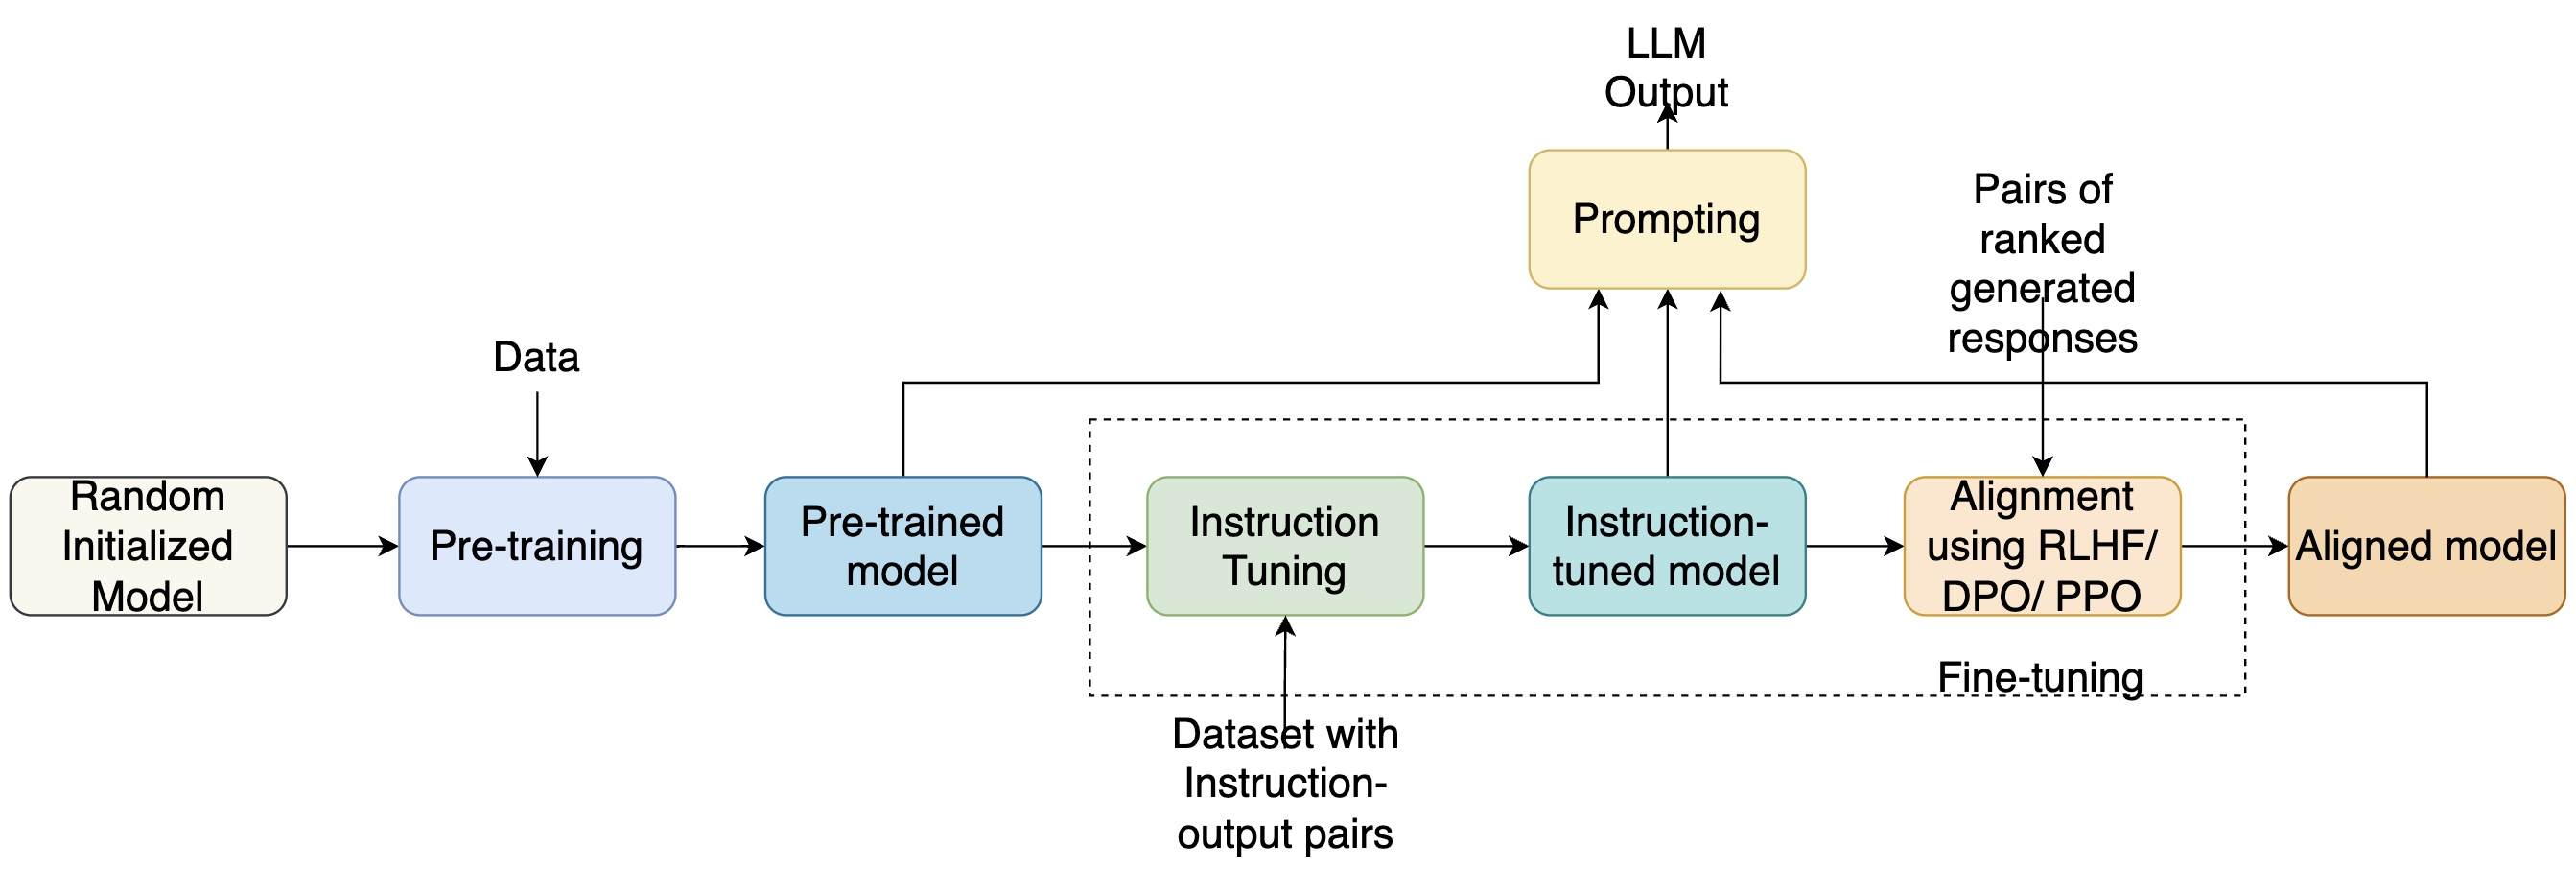
\includegraphics[width=1\textwidth]{Figures/literature_review/llm_training_stages.jpeg} 
    \caption{Various stages of LLM training.}
    \label{fig:LLMTraining}
\end{figure}

\item \textbf{Pre-training.} In the pre-training stage, a model is trained on raw text sequences from large corpora in a self-supervised manner to learn general-purpose representations \cite{dong2019unified}.
\item \textbf{Instruction tuning.} In the instruction tuning stage, LLMs are trained on pairs of instruction-output samples using supervised learning to enhance the model’s ability to respond to specific instructions effectively \cite{shi2024continual}.
\item \textbf{Alignment.} In the alignment stage, LLMs are trained with human feedback to ensure that their generated outputs match human preferences and values. LLM Alignment is important to reduce the risk of the generation of toxic, biased, or undesirable content \cite{shen2023large}.
\end{enumerate}

\subsection{Transformers}
The Transformer architecture, introduced in the paper “Attention is all you need” \cite{vaswani2017attention}, is the fundamental building block of large language models. It uses the attention mechanism, which allows models to selectively focus on different parts of the input sequence at each step of generating an output. Transformers process input in parallel, enabling faster training while effectively capturing long-term dependencies. The transformer architecture usually consists of an encoder stack, which produces a matrix representation for the provided input, and a decoder stack, which generates output iteratively based on the encoded representation. 

\begin{figure}[h]
    \centering
    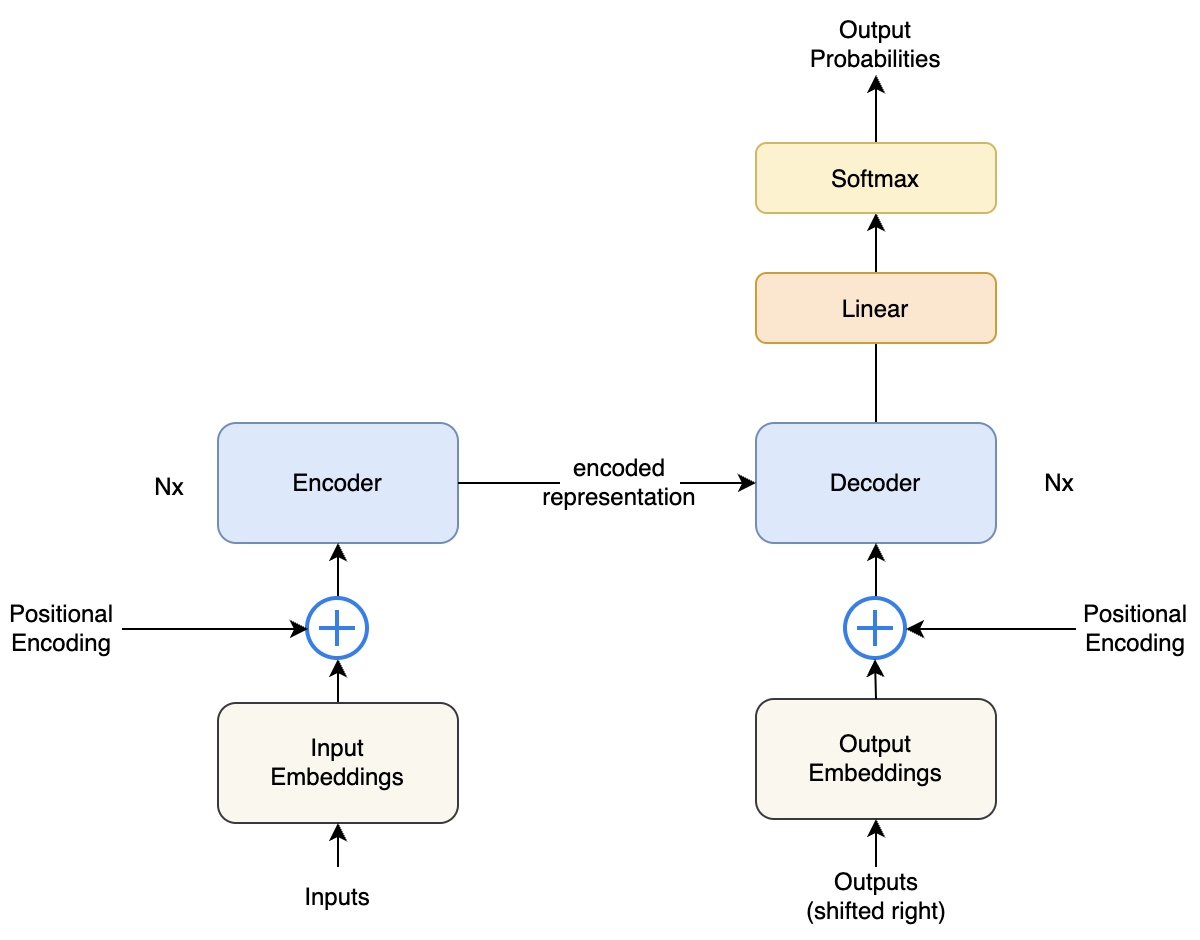
\includegraphics[width=0.75\textwidth]{Figures/literature_review/transformer_architecture.jpeg} 
    \caption{Simplified Transformer Architecture}
    \label{fig:TransformerArchitecture}
\end{figure}

The two key features that make transformers suitable for large language models are positional encodings and self-attention. Positional encodings can be used to encode the position of each word in the input sequence. Positional encodings, provided along with input embeddings, help the model understand the order of the words in an input sequence and thus, generate meaningful output. Self-attention assigns weight to different parts of the input sequence based on their contextual relevance. These features allow the model to learn relationships between different elements over long distances non-sequentially. The ability to process data non-sequentially allows to break down complex problems into smaller computations, making the transformer architecture well-suited for large language models.

\subsection{Auto-regressive models}
Auto-regressive models are a class of models that predict the next component in the sequence based on the measurements from the previous inputs in the sequence. In LLMs, auto-regressive modeling is implemented by using only the decoder stack of the transformer architecture, as seen in Generative Pre-trained Transformer (GPT) models. These models use a causal attention mechanism, where each part can only attend to the previous parts of the sequence.  

The pretraining of the auto-regressive models revolves around predicting the next token in the sequence. This allows the model to learn patterns and dependencies in the language data, making them suitable for tasks that require text generation. Auto-regressive models like OpenAI’s GPT-4, Meta’s Llama models, and Anthropic’s Claude have demonstrated impressive text generation capabilities across a wide range of applications. 

When these auto-regressive models are scaled in size and complexity, these models develop emergent abilities such as zero-shot learning, few-shot learning, and common-sense reasoning as a result of being trained on large amounts of data and increased model capacity \cite{wei2022emergent}. 

\subsubsection{Zero-shot learning} \label{ZeroShot}
Zero-shot learning refers to the ability of the model to perform a task without being provided or shown examples of how to solve the task beforehand.

\subsubsection{Few-shot learning} \label{FewShot}
Few-shot learning refers to the ability of the model to perform new tasks with only a few demonstrations of the task at inference time \cite{brown2020language}. While conventional supervised learning relies on having a large number of labeled samples for training a model on a task, few-shot learning uses transfer learning and meta learning to adapt a pre-trained model on new tasks. Few-shot learning is especially useful when there is a scarcity of labeled samples.

While few-shot learning helps to adapt LLMs to a specific task, it is often necessary to fine-tune a model to achieve better task-specific performance and consistent outputs.


\subsection{Fine-tuning}
Fine-tuning is the process of adapting a pre-trained model for specific tasks or use cases. It uses the extensive knowledge gained by the model which has been pre-trained on a large corpus of data and adapts the model by training it on a smaller, task-specific dataset. It is widely used to update the weights of a pre-trained LLM by training on a supervised dataset for the targeted task \cite{brown2020language}. 

Full fine-tuning involves using techniques like backpropagation and gradient descent to update all model parameters including pre-trained weights by training on task-specific data \cite{xu2023parameter}. The objective is to minimize the task-specific loss, allowing the model to learn patterns from the labeled data. However, this presents two significant challenges:
\begin{enumerate}
\item Updating all model parameters is time-consuming and computationally expensive, especially for larger models.
\item Updating the model parameters to adapt to the new task might lead to degradation of performance on previously learned tasks. This is called catastrophic forgetting.
\end{enumerate}

\subsection{Parameter Efficient Fine-tuning}
Parameter Efficient Fine-Tuning (PEFT) addresses the challenges of full fine-tuning by using different methods to reduce the number of trainable parameters that need to be updated to effectively adapt a pre-trained model to a specific task \cite{xu2023parameter}. PEFT methods update only a small number of additional parameters or update a subset of the pre-trained parameters to adapt the model to the target task while still maintaining comparable performance to full fine-tuning. Since the number of parameters updated is reduced, PEFT methods reduce the risk of catastrophic forgetting. 

\subsection{Low Rank Adaptation (LoRA)} \label{LoRA}
Low Rank Adaptation (LoRA) \cite{hu2021lora} is a type of PEFT method in which the weight changes to the model (\(\Delta W\)) are decomposed into a lower rank representation using low rank transformation. In low rank transformation, a high-dimensional matrix is approximated using a lower-dimensional representation. The rank of a matrix is equal to the number of linearly independent rows (or columns) in it, indicating the minimum number of dimensions required to accurately represent it. Matrix decomposition can be used to represent a larger matrix as a combination of smaller matrices. These matrices can be much smaller than the original matrix but represent the same thing. 

\begin{figure}[h]
    \centering
    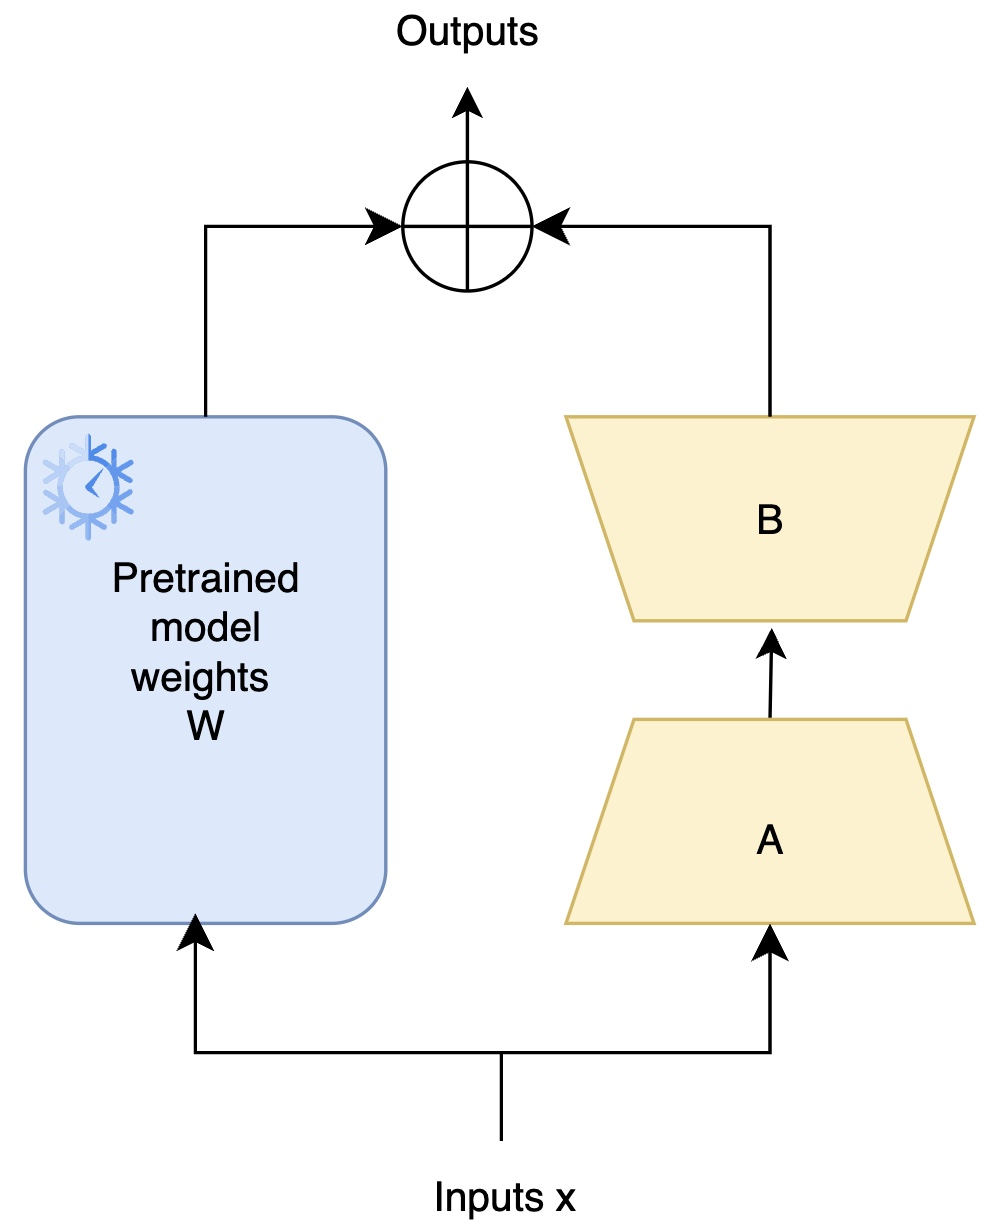
\includegraphics[width=0.5\textwidth]{Figures/literature_review/lora.jpeg} 
    \caption{Fine-tuning with LoRA.}
    \label{fig:LoRA}
\end{figure}

In LoRA, the weight update matrix (\(\Delta W\)) is represented using a product of two decomposed matrices \(W_a\) and \(W_b\) which have a rank of \(r\). The pre-trained model weights are frozen and the trainable rank decomposition matrices are injected into each layer of the transformer architecture. This helps to reduce the number of trainable parameters for adapting to specific downstream tasks. 

\subsection{Instruction Fine-Tuning}
Instruction Fine-tuning \cite{chung2024scaling} is a special form of fine-tuning in which a model is trained on pairs of input-output instructions, enabling the model to learn specific tasks guided by the provided instructions. The aim of instruction fine-tuning is to teach the model to respond to natural language instructions. The intuition behind instruction fine-tuning is that if the model is trained to perform a specific task by training it on instruction data, then the model will learn to follow instructions for unseen tasks as well. Through their evaluation of FLAN \cite{wei2021finetuned}, Jason Wei et al. concluded that instruction fine-tuning substantially improves zero-shot performance on unseen tasks. Instruction fine-tuning reduces the amount of in-context information needed for crafting effective prompts. 
For performing instruction fine-tuning, it is important to prepare a good instruction dataset. Each sample in the instruction dataset should include:
\begin{enumerate}
\item \textbf{Instruction.} A natural language text that specifies the targeted task.
\item \textbf{Input} (optional). Additional text that provides relevant context for the target task. This is optional.
\item \textbf{Output.} The ground-truth value for the provided task based on the provided instruction and context.
\end{enumerate}

\subsection{Continual Learning}
Large Language Models are trained on vast amounts of data using extensive computational resources. However, this knowledge can quickly become outdated, requiring the model to be regularly updated with new knowledge. The immense scale of the LLMs presents a significant challenge for maintaining their relevance in the face of changing data and shifting domains of application \cite{shi2024continual}. Traditional approaches to updating LLMs involve full retraining of the model, which is resource-intensive and computationally expensive. Additionally, this method might lead to the degradation of previously learned information, a phenomenon known as catastrophic forgetting. Continual Learning for LLMs allows the models to learn from a continuous stream of data over time without forgetting previously learned knowledge \cite{wu2024continual}. It aims to develop techniques that allow models to learn new data, adapt to domain shifts, and develop capabilities to perform new tasks while maintaining their broad base of knowledge and capabilities \cite{parisi2019continual}. The successful implementation of continual learning in LLMs can enhance their long-term utility and adaptability, enabling them to remain relevant in an evolving knowledge environment \cite{de2021continual}. Like the training stages of LLMs, continual learning can take place in the following stages:
\begin{enumerate}
\item \textbf{Continual Pre-training.} Continual Pre-training involves regularly updating the models with the latest information and facts, adapting the model to specific domains, and facilitating new language acquisition \cite{gogoulou2023study}. This helps the model to stay up to date with new information and remain relevant across different applications. 
\item \textbf{Continual Instruction Tuning.} Continual Instruction-tuning involves continually fine-tuning LLMs to train the models to learn how to follow instructions and transfer knowledge for future tasks \cite{wu2024continual}. In this stage, models are continually fine-tuned on new instructions or tasks, while maintaining the performance for previously learned tasks.  
\item \textbf{Continual Alignment.} Continual Alignment involves continuously updating LLMs to align with evolving human values, ethics, and data \cite{shi2024continual}. It helps to update LLMs to reflect changes in societal values and integrate new demographic groups to existing LLMs \cite{wu2024continual}. 
\end{enumerate}

In continual learning, one of three scenarios can happen \cite{van2022three}:
\begin{enumerate}
\item The data for different tasks arrives sequentially over time.
\item The data is presented in distinct stages or batches.
\item The underlying distribution of the data gradually changes over time.
\end{enumerate}
Depending on the nature of the change of data, continual learning can be categorized into three types:
\subsubsection{Task-incremental Learning}
In Task-incremental Learning (TIL), a model is sequentially trained to perform a set of distinct tasks over time. In this setting, a task is a well-defined problem or objective characterized by its unique dataset that the model must learn to perform. It must be clear to the model at test time which task must be performed. For this, the different tasks must be clearly defined and separated. In Task-incremental Continual Instruction Tuning, an LLM is continuously fine-tuned on a sequence of task-specific instruction datasets to train the model to perform new tasks \cite{wu2024continual}.  However, research has demonstrated that repeatedly fine-tuning LLMs on data for different tasks can lead to a significant degradation in the performance of previously learned tasks and loss of problem-solving abilities \cite{kotha2023understanding}. Thus, the challenge with task-incremental learning is to find effective ways to prevent catastrophic forgetting and sustain the performance of previously learned tasks when trained on new tasks.
\begin{figure}[h]
    \centering
    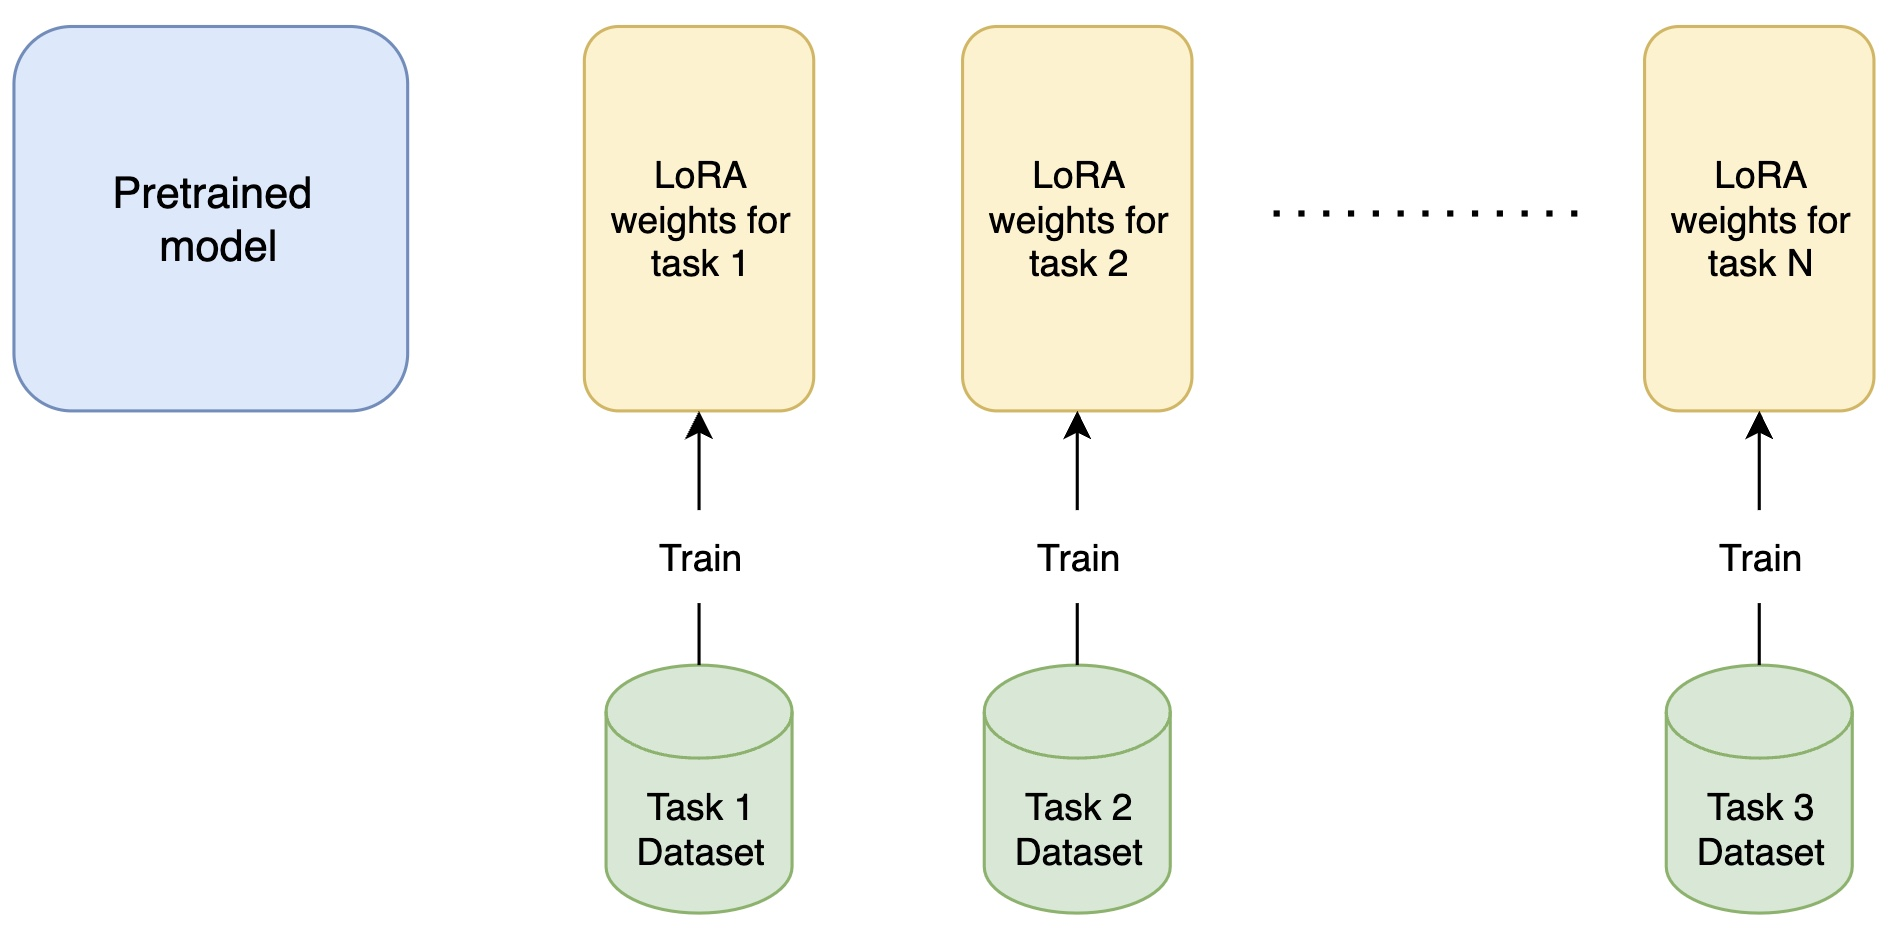
\includegraphics[width=0.75\textwidth]{Figures/literature_review/task_incremental_learning.jpeg} 
    \caption{Task-incremental Learning}
    \label{fig:TaskIncrementalLearning}
\end{figure}

\subsubsection{Domain-incremental Learning}
In Domain-incremental Learning (DIL), the fundamental nature of the problem remains the same but the context or the distribution of input data changes over time. It is characterized by a shift in the domain of application. An example of this is to train an image classification model to recognize a specific object in images with different backgrounds and styles. In Domain-incremental Continual Instruction Tuning, an LLM is trained on a sequence of domain-specific instructions to solve a given task in different domains. 
\begin{figure}[h]
    \centering
    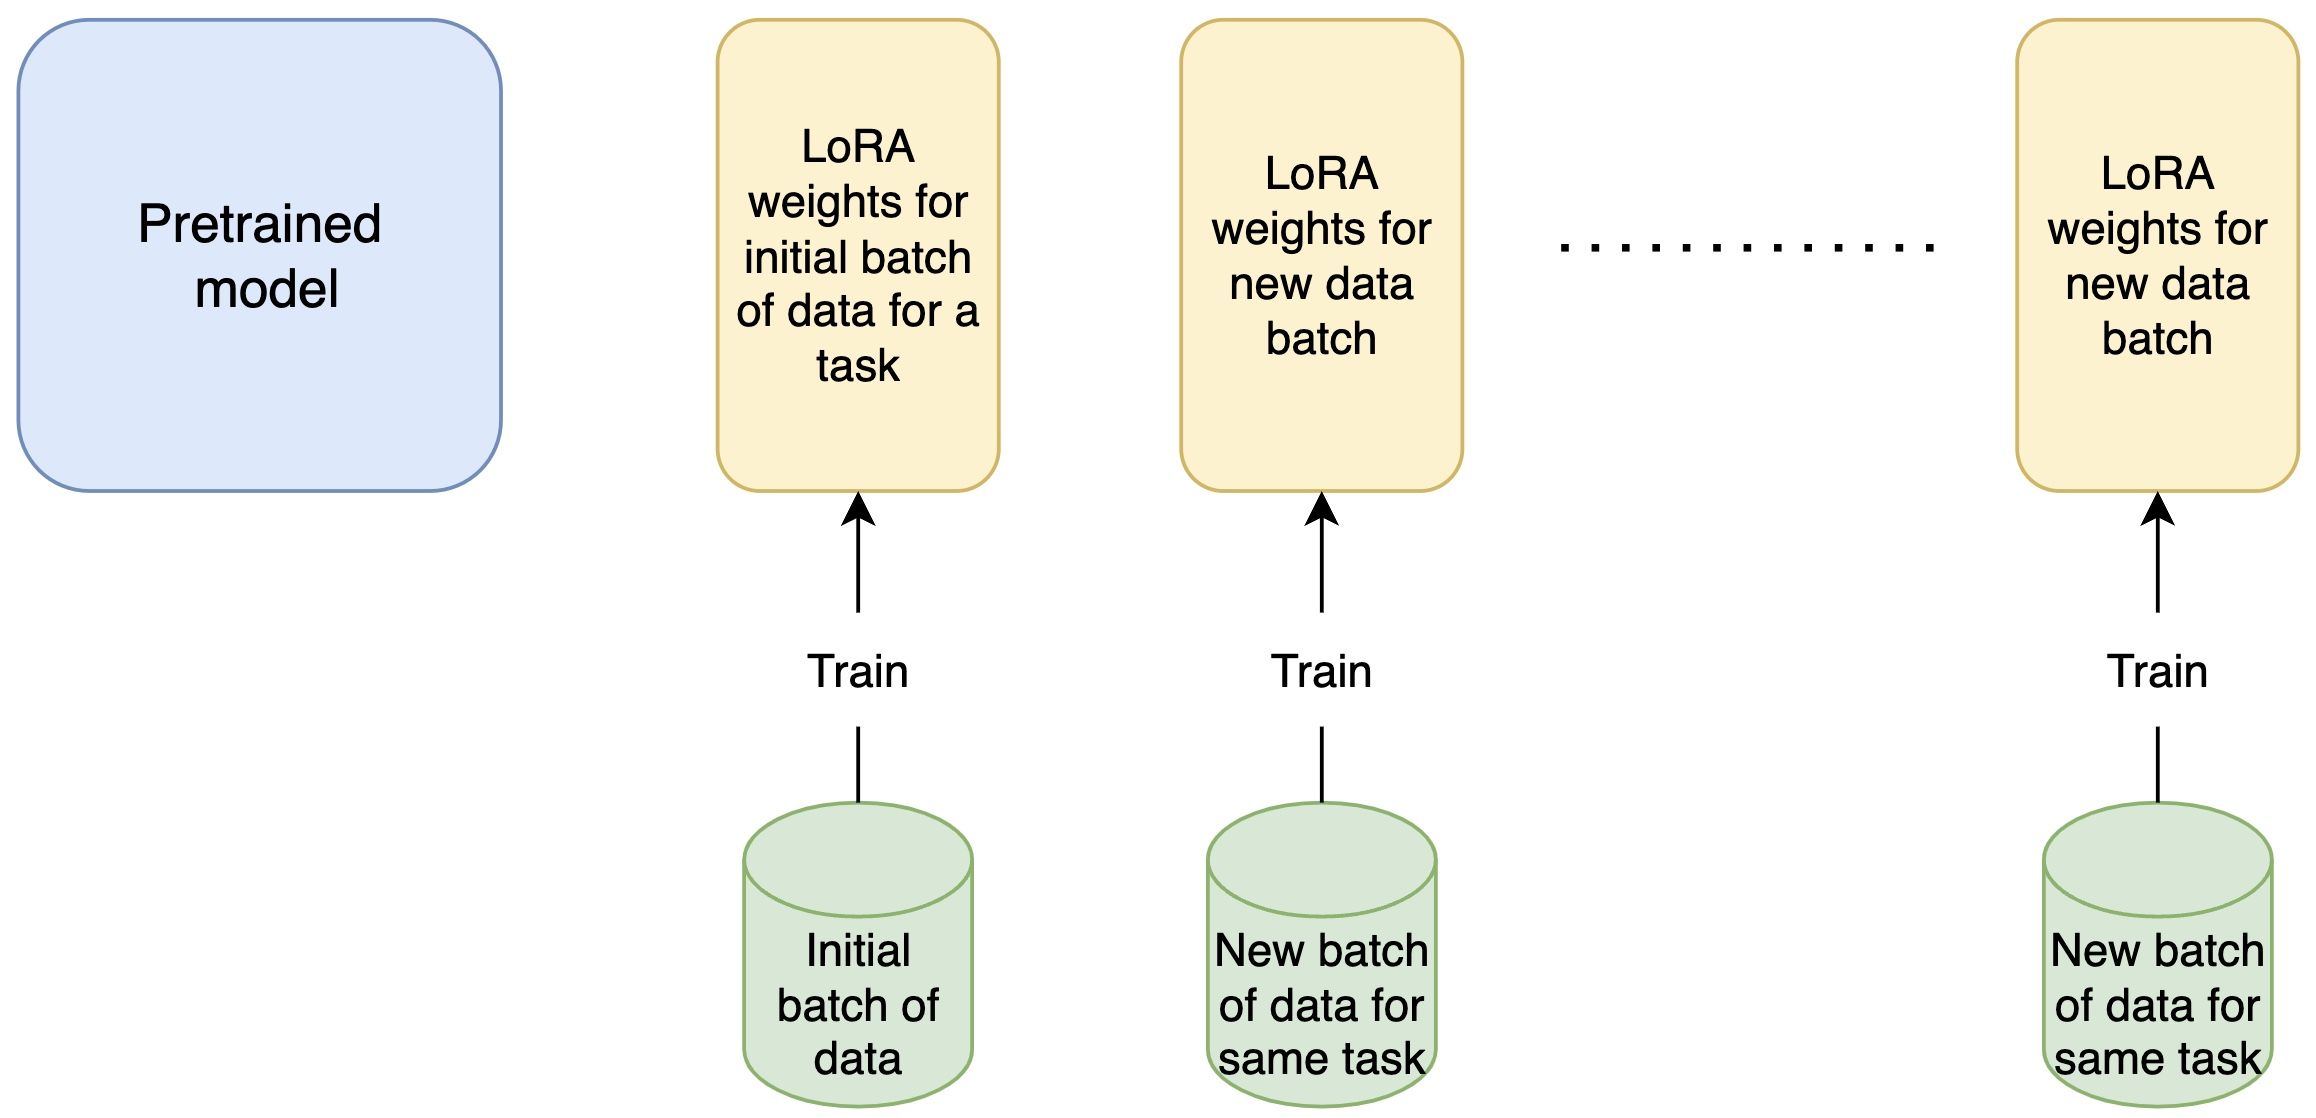
\includegraphics[width=0.75\textwidth]{Figures/literature_review/domain_incremental_learning.jpeg} 
    \caption{Domain-incremental Learning}
    \label{fig:DomainIncrementalLearning}
\end{figure}

\subsubsection{Class-incremental Learning}
In class-incremental Learning (CIT), a model is continuously trained to distinguish between a growing number of objects or classes. Class-incremental learning can be used when we want to train a model on a sequence of classification tasks \cite{rebuffi2017icarl} \cite{von2019continual}. A challenge with class-incremental learning is for the model to be able to identify the set of possible classes that a sample might belong to and thus to be capable of distinguishing sets of classes that do not appear together. 
\begin{figure}[h]
    \centering
    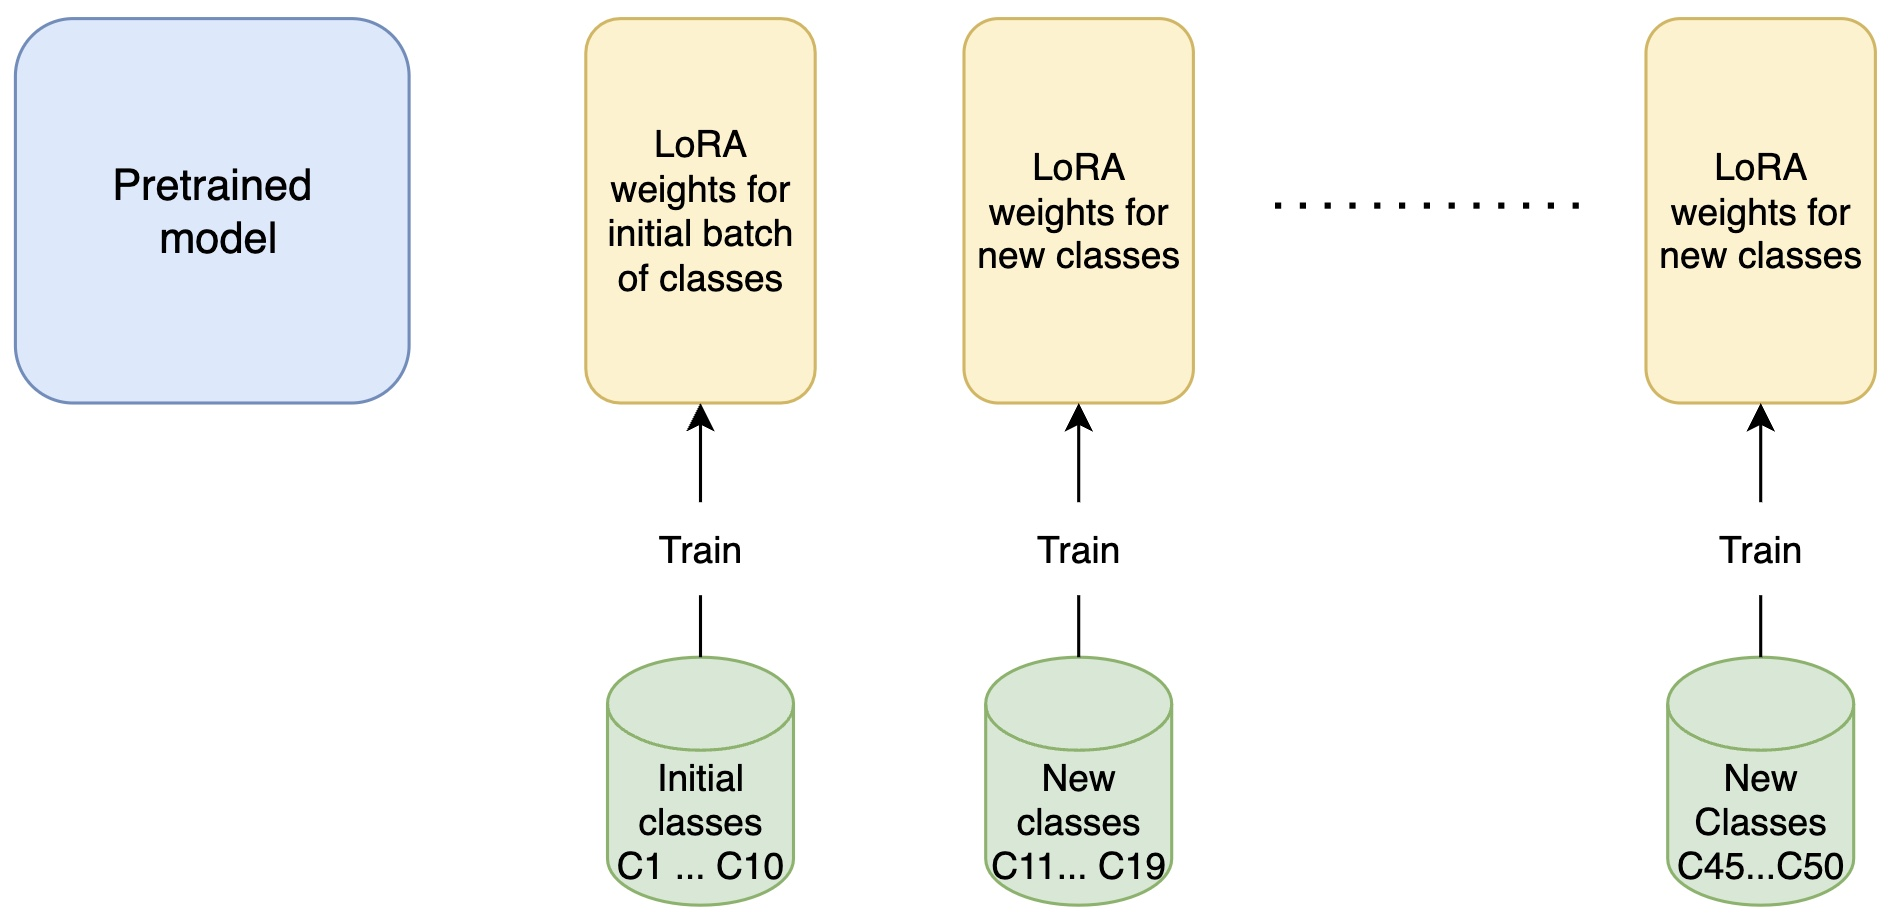
\includegraphics[width=0.75\textwidth]{Figures/literature_review/class_incremental_learning.jpeg} 
    \caption{Class-incremental Learning}
    \label{fig:ClassIncrementalLearning}
\end{figure}

\subsection{Catastrophic Forgetting}
Catastrophic Forgetting is the phenomenon where the performance of a model significantly degrades on previously learned tasks or data when trained on new data \cite{wang2023comprehensive}. Catastrophic Forgetting was introduced in the paper: “Catastrophic interference in connectionist networks: the sequential learning problem” \cite{mccloskey1989catastrophic}. The authors showed that sequentially training neural networks on tasks led the networks to forget previously learned tasks when new tasks are learned. Thus, it is a major challenge in continual learning settings, caused by updates to the model weights when the model adapts to new task environments or data distributions. For instance: when continual pre-training is performed on an instruction fine-tuned model, its ability to follow instructions might be affected.

\section{Related works} \label{RelatedWorks}
In this thesis work, we focus on Task-incremental learning using LoRA-based parameter efficient fine-tuning and investigate the effect of applying replay-based mitigation method for catastrophic forgetting.  To do this, we explored existing mitigation methods that have been proposed to mitigate catastrophic forgetting.  

\subsection{Mitigation methods for catastrophic forgetting} \label{MitigationMethods}
Various approaches have been developed for the mitigation of catastrophic forgetting in continual learning. Depending on the way the task-specific information is stored and used, these mitigation approaches have been classified into three categories \cite{de2021continual}:

\subsubsection{Replay-based methods} \label{Replay}
In replay-based methods, a memory buffer is used to store the samples from the previous tasks. The samples can be either directly taken from the task dataset, or the trained model can be used to generate pseudo samples for a specific task. These samples are replayed when training the model on a new task to mitigate forgetting. The data from the memory buffer can be used in two ways \cite{de2021continual}:

\paragraph{Rehearsal-based methods} \label{Rehearsal} In rehearsal-based methods, the replay buffer is combined with the training data for the new task during the learning process. The key challenge for rehearsal methods is the proper construction and use of the memory buffer \cite{wang2024comprehensive}. To ensure effective performance, the samples from the previous tasks must be carefully selected to recover previous task capabilities. Chaudhry et al. \cite{chaudhry2019tiny} explored Reservoir Sampling, Ring Buffer, k-means, and Means of Features (MoF) as sample selection strategies. Reservoir Sampling takes a stream of input and returns a random subset of items from that stream. The Ring Buffer allocates an equal number of training samples per class. K-means is used to identify the k-centroids of the representations in the feature space and then populate the memory buffer with samples whose feature representation is closest to the centroids. Means of Features selects an equal number of samples that are close to the feature mean for each task/ class. Quality-Focused Data Selection is introduced in Cognitive Replay (CORE) \cite{zhang2024core} (Section \ref{Core}) to select representative samples from each task to populate the memory buffer. The quantity of the data selected also affects the efficacy of the memory buffer. Continual-T0 \cite{scialom2022fine} used 1\% of data of the learned task for the rehearsal buffer while ConPET \cite{song2023conpet} used a dynamic sampling strategy and removed the fixed storage space limit for the buffer. Dual-stage Mixed Fine-tuning (DMT) \cite{dong2023abilities} looked at how data composition in the replay buffer affects the model performance and concluded that mixing data sources in supervised fine-tuning improves performance in low-resource scenarios and diminishes performance in high-resource scenarios. 

When the data from previously learned tasks is not accessible, pseudo rehearsal can be used. This involves using the trained model to approximate the training data for the previous tasks. This is also called generative replay \cite{wang2024comprehensive}. Recent studies have shown the effectiveness of generative models to generate high-quality samples that model the distribution of the training samples \cite{shin2017continual}. However, the performance of generative replay heavily depends on the quality of the generative model used. Despite their simplicity, rehearsal-based methods are found to be effective, even with a small episodic memory \cite{shi2024continual}. Dark Experience Replay (DER++) \cite{buzzega2020dark} was found to show improved performance with the use of a small rehearsal buffer. However, the performance of rehearsal methods is dependent on how the joint training of the previous tasks and the new task performs \cite{de2021continual}.

\paragraph{Constrained Optimization methods} The memory buffer can be used to constrain the loss function for the new task, minimizing the interference with previously learned tasks. The model parameter updates are constrained to align with the direction of the rehearsal buffer to preserve the previous input and gradient space \cite{de2021continual}. This is done in Gradient Episodic Memory (GEM) \cite{lopez2017gradient} by performing gradient projection, where the estimated gradient direction is projected on the feasible region delineated by task gradients for previously learned tasks through first-order Taylor Series approximation \cite{wang2024comprehensive}. Average GEM (A-GEM) \cite{chaudhry2018efficient} simplifies this by projecting on one direction estimated by randomly selected samples from the memory buffer for a previous task. 

Orthogonal Gradient Descent (OGD) \cite{farajtabar2020orthogonal} attempts to mitigate catastrophic forgetting by projecting the gradients for the new task onto a subspace in which the outputs of the network on the previous tasks do not change. Similarly, techniques like Orthogonal Weights Modification (OWM) \cite{zeng2019continual} and Adaptive Orthogonal Projection (AOP) \cite{guo2022adaptive} use orthogonal projection for dealing with catastrophic forgetting. Orthogonal projection involves learning each task by updating the network parameters in a direction orthogonal to the previously learned task subspaces, ensuring no interference between tasks.

In this thesis work, we investigate the effectiveness of the replay-based mitigation method. In particular, we used the CORE \cite{zhang2024core} replay method, which is discussed in extensive detail below:
\paragraph{Cognitive Replay (CORE)} \label{Core}
Cognitive Replay (CORE) \cite{zhang2024core} is a rehearsal-based mitigation method for catastrophic forgetting in continual learning. CORE uses a fixed-sized memory buffer for replay. To improve the efficiency of the replay buffer. CORE introduces two strategies derived from human cognition review processes: Adaptive Quantity Allocation (AQA) for dynamically determining the buffer space allocated for each task and Quality-Focused Data Selection (QFS) for selecting more representative samples from each task to populate the buffer. 
\begin{figure}[h]
    \centering
    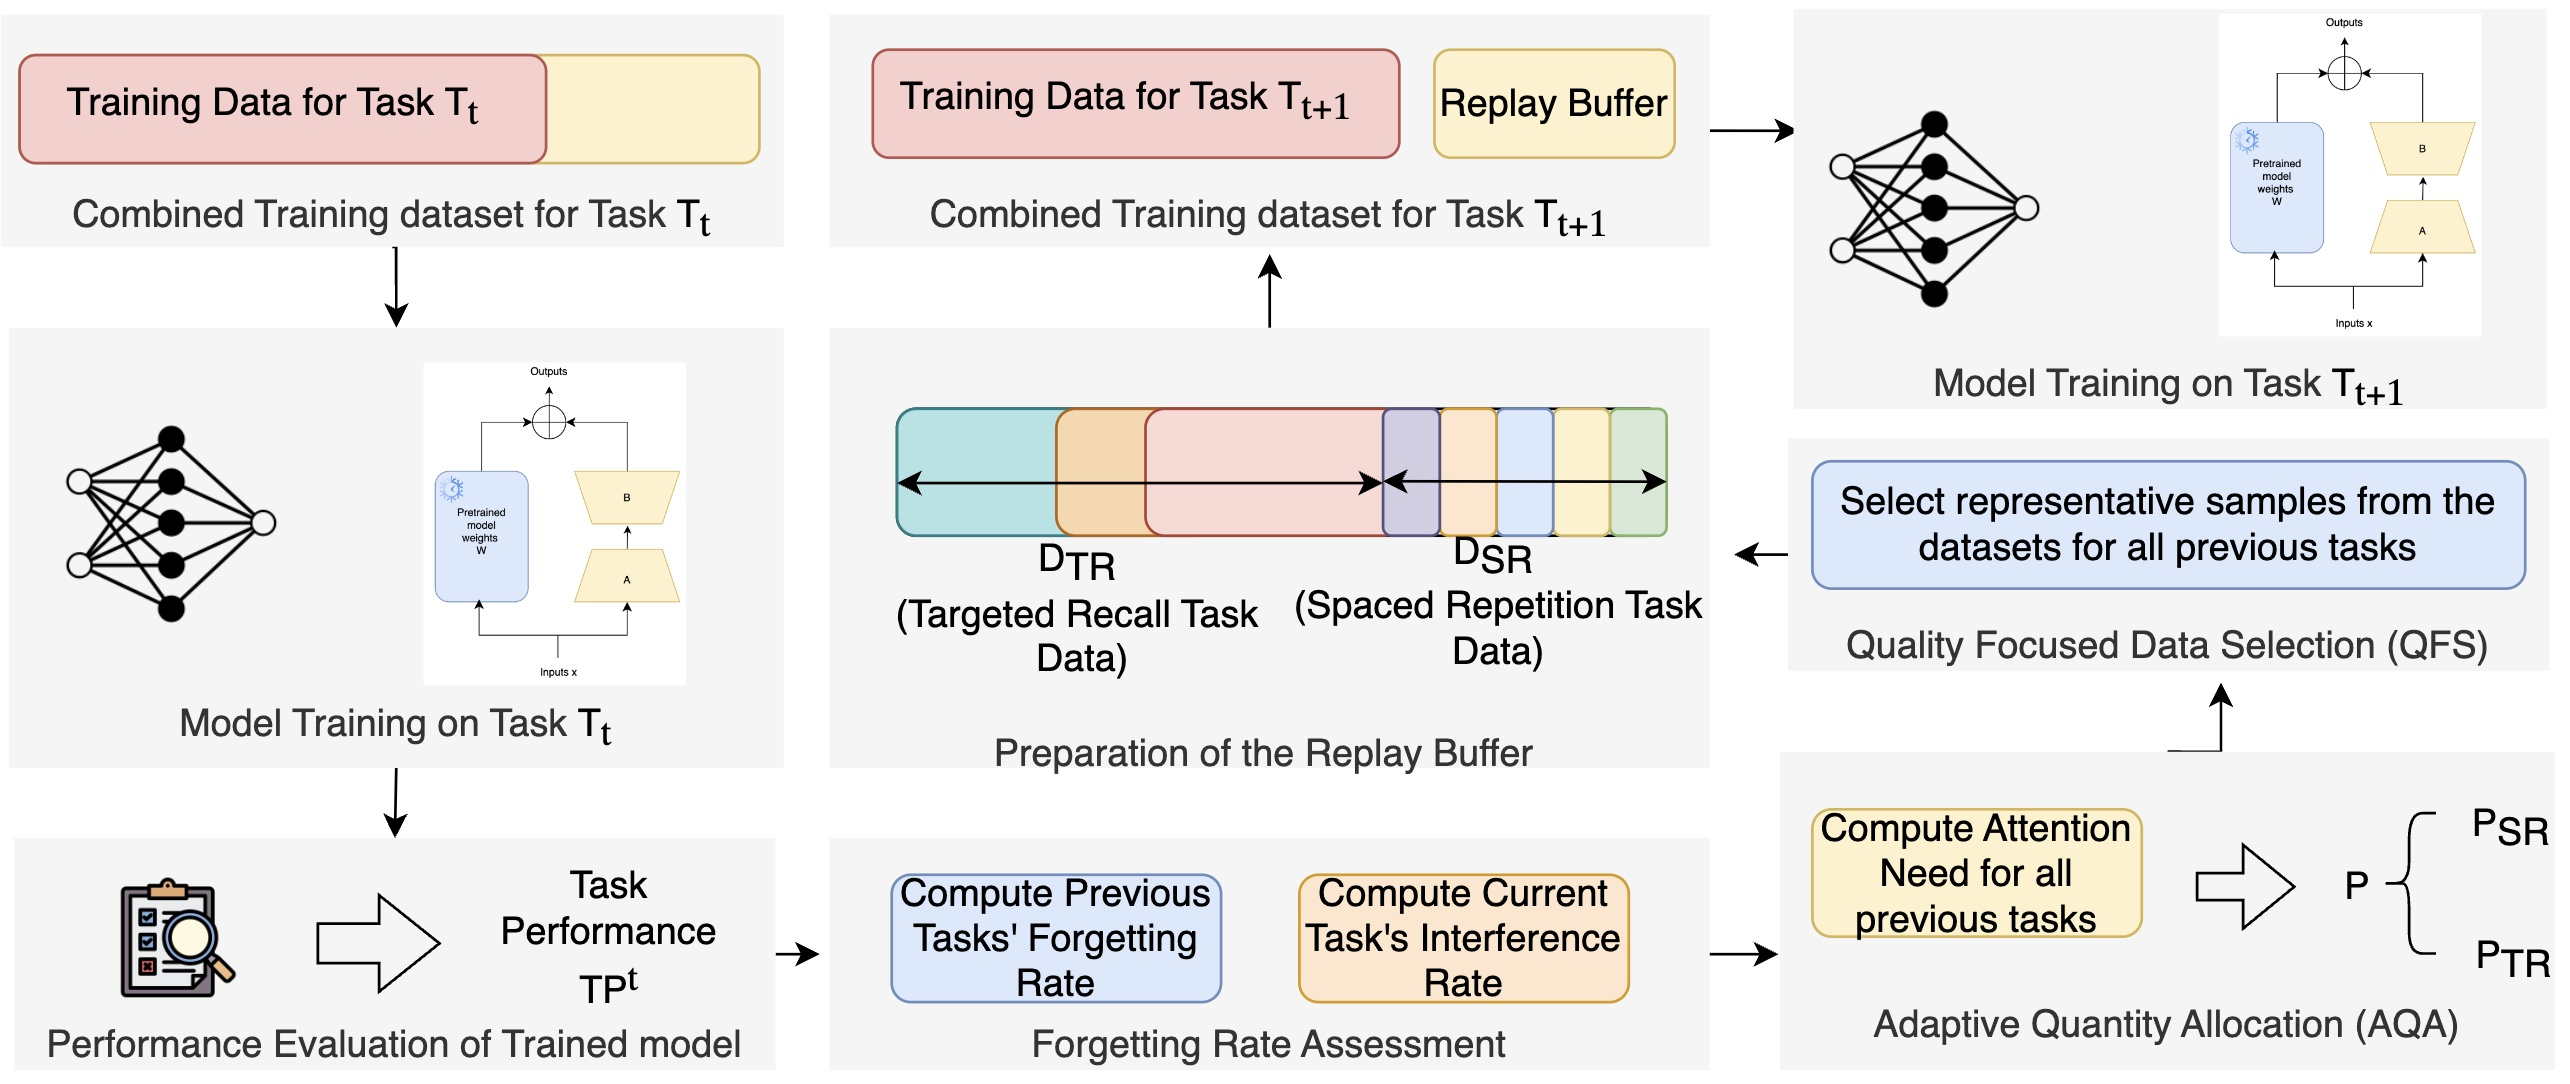
\includegraphics[width=1\textwidth]{Figures/literature_review/core_replay_process.jpeg} 
    \caption{Cognitive Replay (CORE) Process Pipeline}
    \label{fig:CoreReplay}
\end{figure}
\subparagraph{Adaptive Quantity Allocation.} \label{AQA} Buffer space allocation is done based on the attention need of the task. The attention required for the task is computed by using the forgetting rate and interference rate of each task.
\begin{enumerate}
\item \textbf{Forgetting Rate.} The forgetting rate of a task is the difference between the peak performance of the model on the task and its current performance. After fine-tuning the model on a task, the performance of the model on all the completed tasks is evaluated and the forgetting rate is computed. For a task p, the forgetting rate is calculated as:
\begin{equation} \label{ForgettingRate}
f_p = \max_{i \in \{1, 2, \ldots, \tau - 1\}} \left( \text{TP}_p^i - \text{TP}_p^\tau \right) \quad \text{for} \quad p \in P
\end{equation}

Where:
\begin{itemize}
    \item \( f_p \) is the forgetting rate for task \( p \).
    \item \( \tau \) is the last fine-tuned task.
    \item \(\text{TP}\) is the task performance for task \( p \).
    \item \( P \) is the set of all completed tasks.
\end{itemize}

\item \textbf{Interference Rate.} The interference rate, which is the measure of the influence of the buffer data on the last fine-tuned task, is computed as:
\begin{equation} \label{InterferenceRate}
i_p = \frac{e^{\text{TP}_p^{\tau-1} - \text{TP}_p^\tau}}{\sum_{p' \in P} e^{\text{TP}_{p'}^{\tau-1} - \text{TP}_{p'}^\tau}} \quad \text{for} \quad p \in P
\end{equation}

Where:
\begin{itemize}
    \item \( i_p \) is the interference rate for task \( p \).
\end{itemize}

\item \textbf{Attention-based Allocation.} The attention needed for a task tells us which task requires more attention and therefore more space in the memory buffer. For all previous tasks: tasks 1 to \( \tau \)-1, attention is computed using the forgetting rate of the task.
\begin{equation} \label{attention}
a_p = -\log(1 - f_p) \quad \text{for} \quad p \in P, \, f_p \in F_P
\end{equation}
Where:
\begin{itemize}
    \item \( a_p \) is the attention score for previous task \( p \).
\end{itemize}

For the last fine-tuned task \( \tau \), the attention score is computed using the forgetting rate and the interference rate.
\begin{equation} \label{attention2}
a_p = -\log\left(1 - \sum_{i}^{\tau-1} f_i \cdot i_i \right) \quad \text{for} \quad p \in P, \, f_p \in F_P, \, i_p \in I_P
\end{equation}
Where:
\begin{itemize}
    \item \( a_p \) is the attention score for the last fine-tuned task \( p \).
\end{itemize}

The calculated attention score is then normalized using softmax:
\begin{equation} \label{normalized_threshold}
a_p^s = \frac{e^{a_p}}{\sum_{i \in P} e^{a_i}} \quad \text{for} \quad p \in P
\end{equation}

The normalized attention score for a task is then compared against a threshold value to determine whether the task is a Targeted Recall (TR) or a Spaced Repetition (SR) task. Targeted Recall tasks are those that require more attention and hence more space in the memory buffer. In contrast, Spaced Repetition tasks are those that require the bare minimum attention. The threshold value is computed as:
\begin{equation} \label{threshold}
a_t = \frac{1}{\lambda \cdot |P|}
\end{equation}
Where:
\begin{itemize}
    \item \(a_t\) is the attention threshold.
    \item \(\lambda\) is the replay lambda parameter.
    \item \(|P|\) is the count of the total completed tasks.
\end{itemize}

\begin{equation} 
p \in \left\{
\begin{array}{ll}
P_{SR}, & \text{if } a_p^s \leq a_t \\
P_{TR}, & \text{if } a_p^s > a_t
\end{array}
\right.
\end{equation}
Where:
\begin{itemize}
    \item\( P_{SR} \) is the set of Spaced Repetition tasks.
    \item \( P_{TR} \) is the set of Targeted Recall tasks.
\end{itemize}

To ensure that the Spaced Repetition tasks get an attention score that would be useful, all Spaced Repetition tasks are assigned a minimum attention score.
\begin{equation} \label{minimum_attention}
\text{minimum attention (a}_{\text{SR}}\text{)}= \frac{1}{\lambda * |P_{\text{SR}}|}
\end{equation}
The remaining attention is then allocated to the Targeted Recall tasks:
\begin{equation} \label{TRattention}
(a_p) = \left(1 - \frac{|P_{SR}|}{\lambda \cdot |P|}\right) \left(\frac{a_p^s}{\sum_{p' \in P_{TR}} a_{p'}^s}\right), \text{ if } p \in P_{TR}
\end{equation}

Where:
\begin{itemize}
    \item $|P_{SR}|$ is the number of spaced repetition tasks and $|P|$ is the total number of tasks.
\end{itemize}

The buffer space is then computed using:
\begin{equation} \label{bufferspace}
\text{Task Buffer Space}(D_p) = a_p \times \text{Buffer size}
\end{equation}
\end{enumerate}

\subparagraph{Quality-Focused Data Selection.} CORE uses the following algorithm to select more representative samples from each task:
\begin{enumerate}
\item Select a random sample from the dataset of a specific task.
\item Select a subsequent sample that minimizes the distance between the average feature representation of the previously selected sample and the average feature representation of the entire task dataset in the feature space.
\end{enumerate}

Through their experiments on classification task with split-MNIST and split-CIFAR image datasets, the authors demonstrated that CORE replay achieves the highest average task accuracy and performs better on the tasks that are susceptible to forgetting.

\subsubsection{Regularization-based methods}
In regularization-based methods, an extra regularization term is added to the loss function to balance previously learned and new tasks \cite{de2021continual}. The added regularization term helps to consolidate knowledge from previously learned tasks when training the model on a new task. These methods help to maintain privacy by removing the need to store raw task data and consequently reduce memory requirements. Depending on the focus of regularization, these methods can be categorized into:

\paragraph{Data-focused methods} 
Data-focused methods use different techniques to retain important data instances from previous tasks while learning new tasks. These methods primarily use Knowledge Distillation, where the previously learned model is treated as the teacher and the model being trained on new data is treated as the student to mitigate catastrophic forgetting \cite{de2021continual}. The target of knowledge distillation should include all training samples from previously learned tasks. 

Learning without Forgetting (LwF) \cite{li2017learning} is a data-focused method that retains knowledge from previous tasks by distilling it into a separate network, allowing the model to learn new tasks while preserving the knowledge from the previous tasks. In LwF, we have a network that can perform previously learned tasks and the objective is to teach this model to perform a new task without forgetting learned tasks. To do this, the new data is presented to the model and its responses to the new data for the old tasks are stored. New nodes are added for training the model on the new task, and the training is done such that only the new nodes are trained at first to minimize the loss for all tasks using the added regularization term with stochastic gradient descent. Then all the weights are jointly trained until convergence. The training is performed such that the model learns to provide correct answers on the new data for the newly trained task and provides the previously stored answers for the older tasks. This allows the model to learn new tasks while preserving capabilities from previous tasks without having to review previous data.

\paragraph{Prior-focused methods}
Prior-focused methods constrain the parameters of a model to stay close to their previous values when learning a new task \cite{de2021continual}. The main concept behind prior-focused methods is to limit changes to important parameters of the model to preserve the knowledge of previously learned tasks. In prior-focused methods, a regularization term is added to the loss function, which penalizes changes to parameters that were important for previous tasks. The important parameters are identified based on their contribution to the performance of previous tasks. Unlike data-focused methods, prior-focused methods constrain the model parameters directly. 

In Elastic Weight Consolidation (EWC) \cite{kirkpatrick2017overcoming}, Fisher’s information matrix is used to estimate the importance of parameters for previously learned tasks. A quadratic penalty is added to the loss function to constrain updates and prevent significant changes to the important parameters. The penalty should be greater for those parameters whose values considerably affect the performance on previous tasks. The addition of the quadratic constraint leads to less forgetting in a continual learning implementation with supervised learning. Online EWC \cite{schwarz2018progress} uses the running sum of Fisher’s matrices, improving EWC and making it suitable to handle longer sequences of text. 

In Variational Continual Learning (VCL) \cite{nguyen2017variational}, the model’s understanding of the world is updated by being trained on new data while preserving its knowledge from previous data. The model’s knowledge is represented as a probability distribution over its parameters. When trained on a new task, the goal is to find a new distribution that matches the old one and performs well on the new task. Although regularization methods normally do not require storing raw data from older tasks, VCL maintains a small set of samples from previously learned tasks, like replay-based methods. 

\subsubsection{Parameter-isolation methods}
In Parameter-isolation methods, separate sets of model parameters are allocated to each task to prevent task interference and catastrophic forgetting \cite{de2021continual}. These methods either add new layers for new tasks, while keeping the parameters for previously learned tasks frozen or ensure that different parts of the network are allocated to the different tasks. Some parameter isolation methods are described as follows:

In Progressive Neural Networks \cite{rusu2016progressive}, a pool of pretrained models is retained throughout training to learn lateral connections from them through adapters to extract useful features for the new task. A Progressive Network starts with a single column with a deep neural network. This network is trained on a specific task. When switching to a second task, the parameters for the first task are frozen and a new column is added where the layers of the new network can receive input via lateral connections from the previous network. This ensures that the model capability to perform previously learned tasks is preserved since their columns are not changed. It also enables knowledge transfer since the new columns receive input from the old columns for faster learning. Using this strategy, Progressive Networks mitigate catastrophic forgetting. However, this method might lead to memory issues when using continual learning for a large number of tasks.

Progressive Prompts \cite{razdaibiedina2023progressive} uses soft-prompt tuning as a parameter isolation strategy to learn new tasks without forgetting previous ones. In this method, a separate prompt is learned for each new task and sequentially concatenated with previously learned prompts, while keeping the model parameters frozen. For a new task, a new prompt is created and prepended to all the existing prompts that have been learned. This combined prompt is added in front of the input text. The training is done only on the new prompt, keeping the previous prompts and the model weights frozen. This ensures that the capabilities learned for previous tasks are preserved. Since the new prompt is prepended in front of the set of older prompts, the new task can benefit from the prompts learned for the previous tasks. 
\begin{figure}[h]
    \centering
    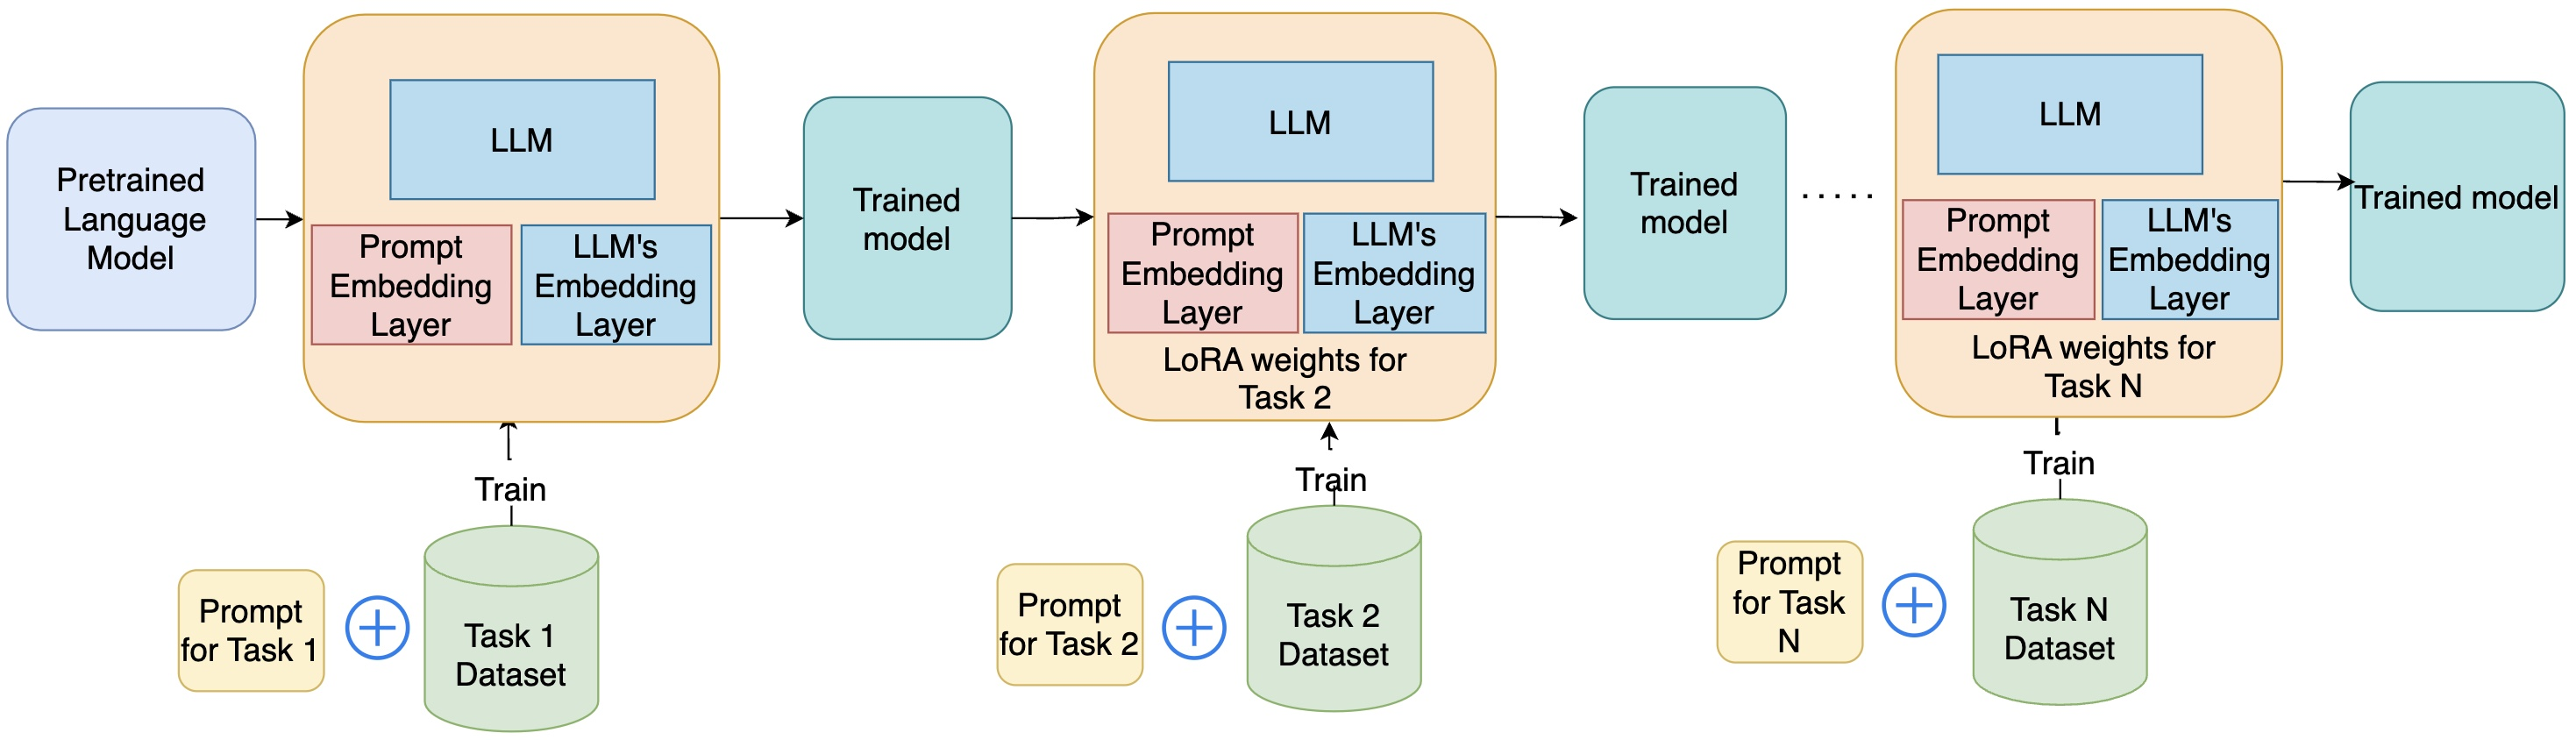
\includegraphics[width=1\textwidth]{Figures/literature_review/progressive_prompt.jpeg} 
    \caption{Progressive Prompts}
    \label{fig:ProgressivePrompts}
\end{figure}

Continual Learning with Low Rank Adaptation (CoLoR) \cite{wistuba2023continual} is a LoRA (Section \ref{LoRA}) based parameter isolation method for continual learning. For each new task, CoLoR trains a LoRA adapter and creates an expert model for each dataset. A suitable loss function is used for each task. Using LoRA-based fine-tuning ensures that the base model parameters are intact and remain unaffected by the training for the new task. A separate model for each task ensures that there is no task interference. During training, k-means clustering is performed on the features of the training data to identify k representative points for each dataset. During inference, dataset identification is performed by finding which representative points closely match the provided input. The expert model for the identified dataset is used for inference. Through their experiments on image classification tasks, the authors demonstrated that ColoR outperforms prompt tuning in domain and class-incremental learning. 
\begin{figure}[h]
    \centering
    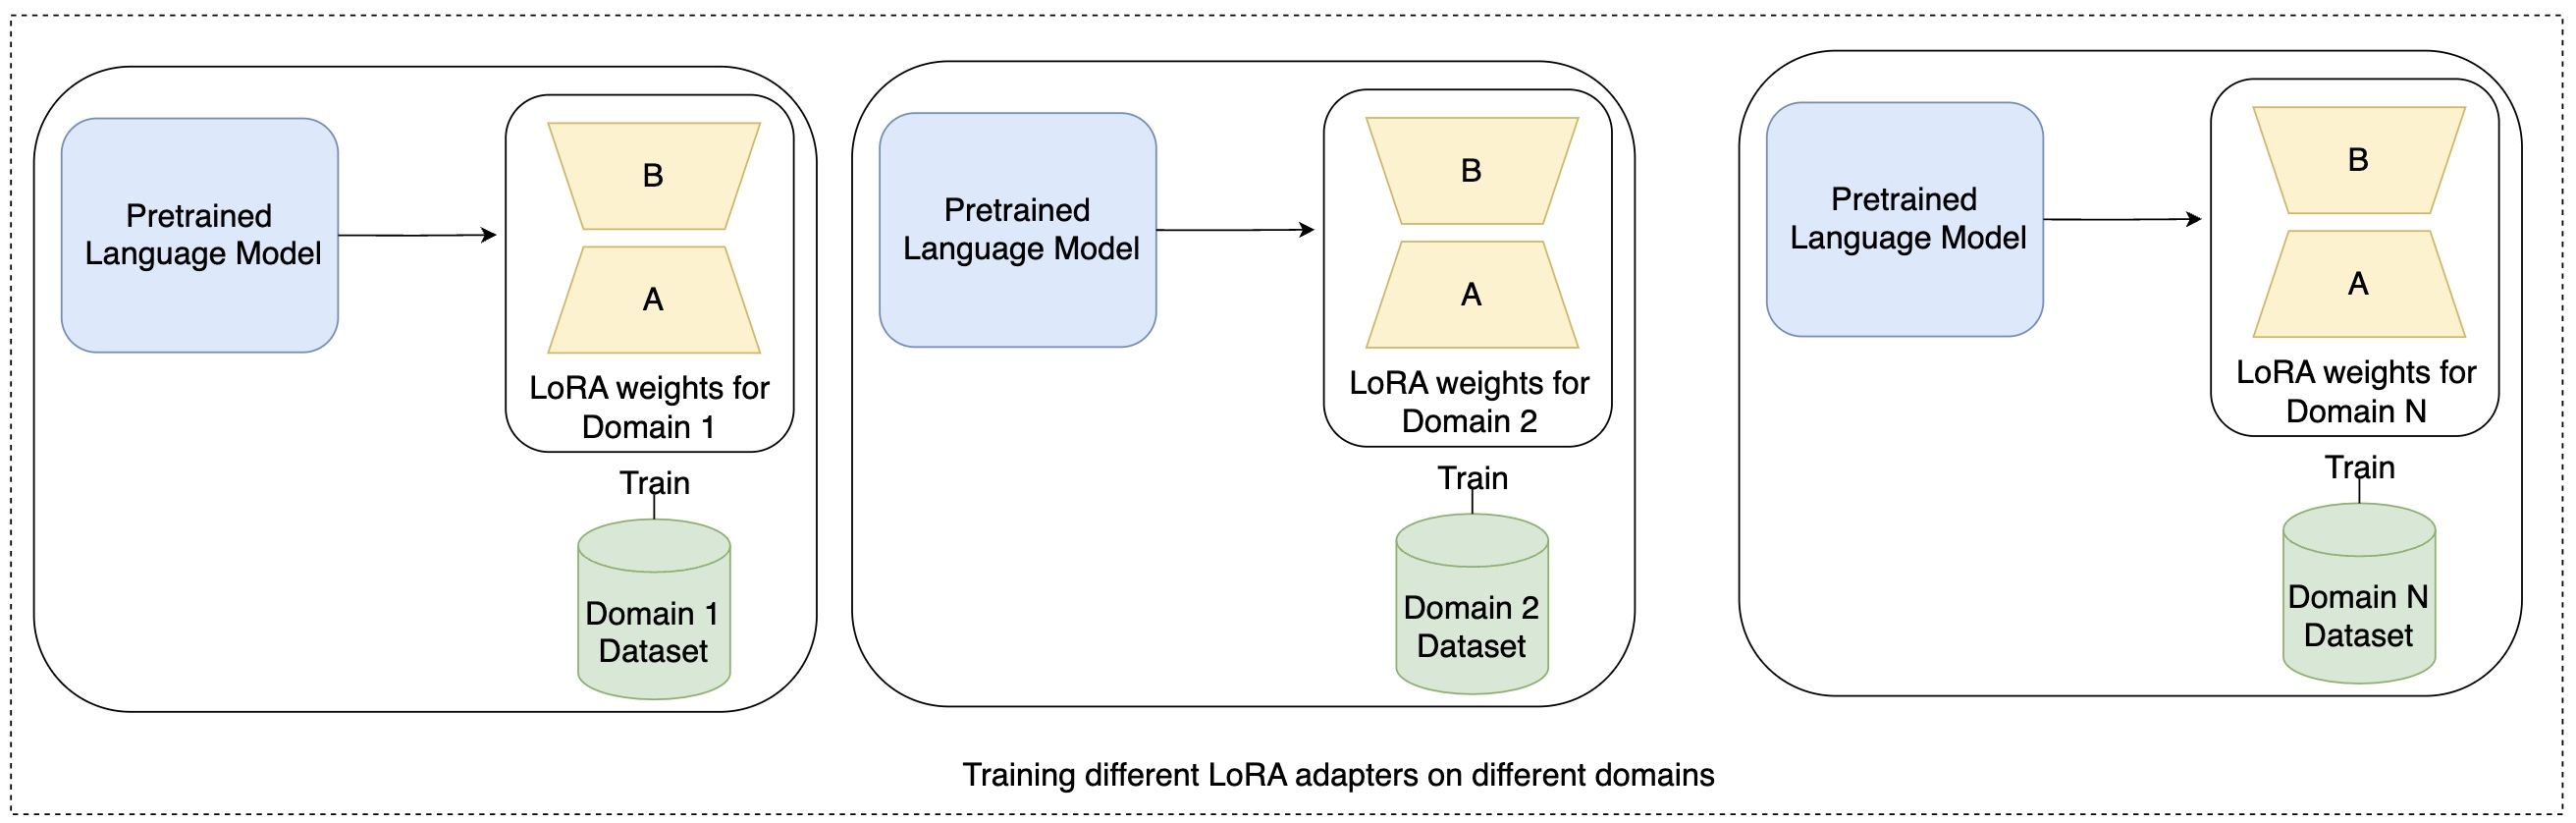
\includegraphics[width=1\textwidth]{Figures/literature_review/CoLoR.jpeg} 
    \caption{Continual Learning with Low Rank Adaptation}
    \label{fig:Color}
\end{figure}

\subsubsection{Hybrid methods}
Existing methods also use a combination of elements from different mitigation approaches. This hybrid approach allows using the strengths of different techniques while also mitigating their weaknesses. Some methods that use a hybrid approach include:

Lifelong Few-shot Language Learning with Prompt Tuning of T5 (LFPT5) \cite{qin2021lfpt5} is a framework for continual learning based on prompt tuning. This method uses prompt tuning with few-shot learning and trains the model on text-to-text tasks such as Named Entity Recognition (NER), Classification, Summarization, and Question Answering. While training, the prompt embeddings are trained as both a task solver and a data generator. LFPT5 is a hybrid approach that uses a combination of prompt tuning as a parameter isolation approach and generative replay as a replay-based approach. When introducing a new domain to the model, it first generates pseudo-labeled samples of previously learned domains. Similar to rehearsal-based methods, these generated samples are added to the training data for the new domain to mitigate catastrophic forgetting. Using their experiments on task-incremental and domain-incremental learning, the authors demonstrated that LFPT5 can generalize on new few-shot tasks without severely degrading the model’s capabilities on previously learned tasks and domains. 

Orthogonal LoRA (O-LoRA) \cite{wang2023orthogonal} is a hybrid approach for continual learning that combines regularization method and LoRA, which is a parameter isolation method. O-LoRA uses LoRA-based parameter efficient fine-tuning to train the model. Thus, it requires only small changes to the parameters of the model when being trained on a new task. O-LoRA learns each task in a different vector sub-space. These vector subspaces are kept orthogonal to each other to minimize interference between tasks. O-LoRA uses instruction fine-tuning as the training method. 

Learning-Accumulation-Ensemble (LAE) \cite{gao2023unified} is a unified continual learning framework that uses parameter efficient tuning to adapt a pre-trained model to a specific task. This framework is compatible with different PEFT methods including Adapter tuning, LoRA, and Prefix tuning. The three main components of the framework are:
\begin{figure}[h]
    \centering
    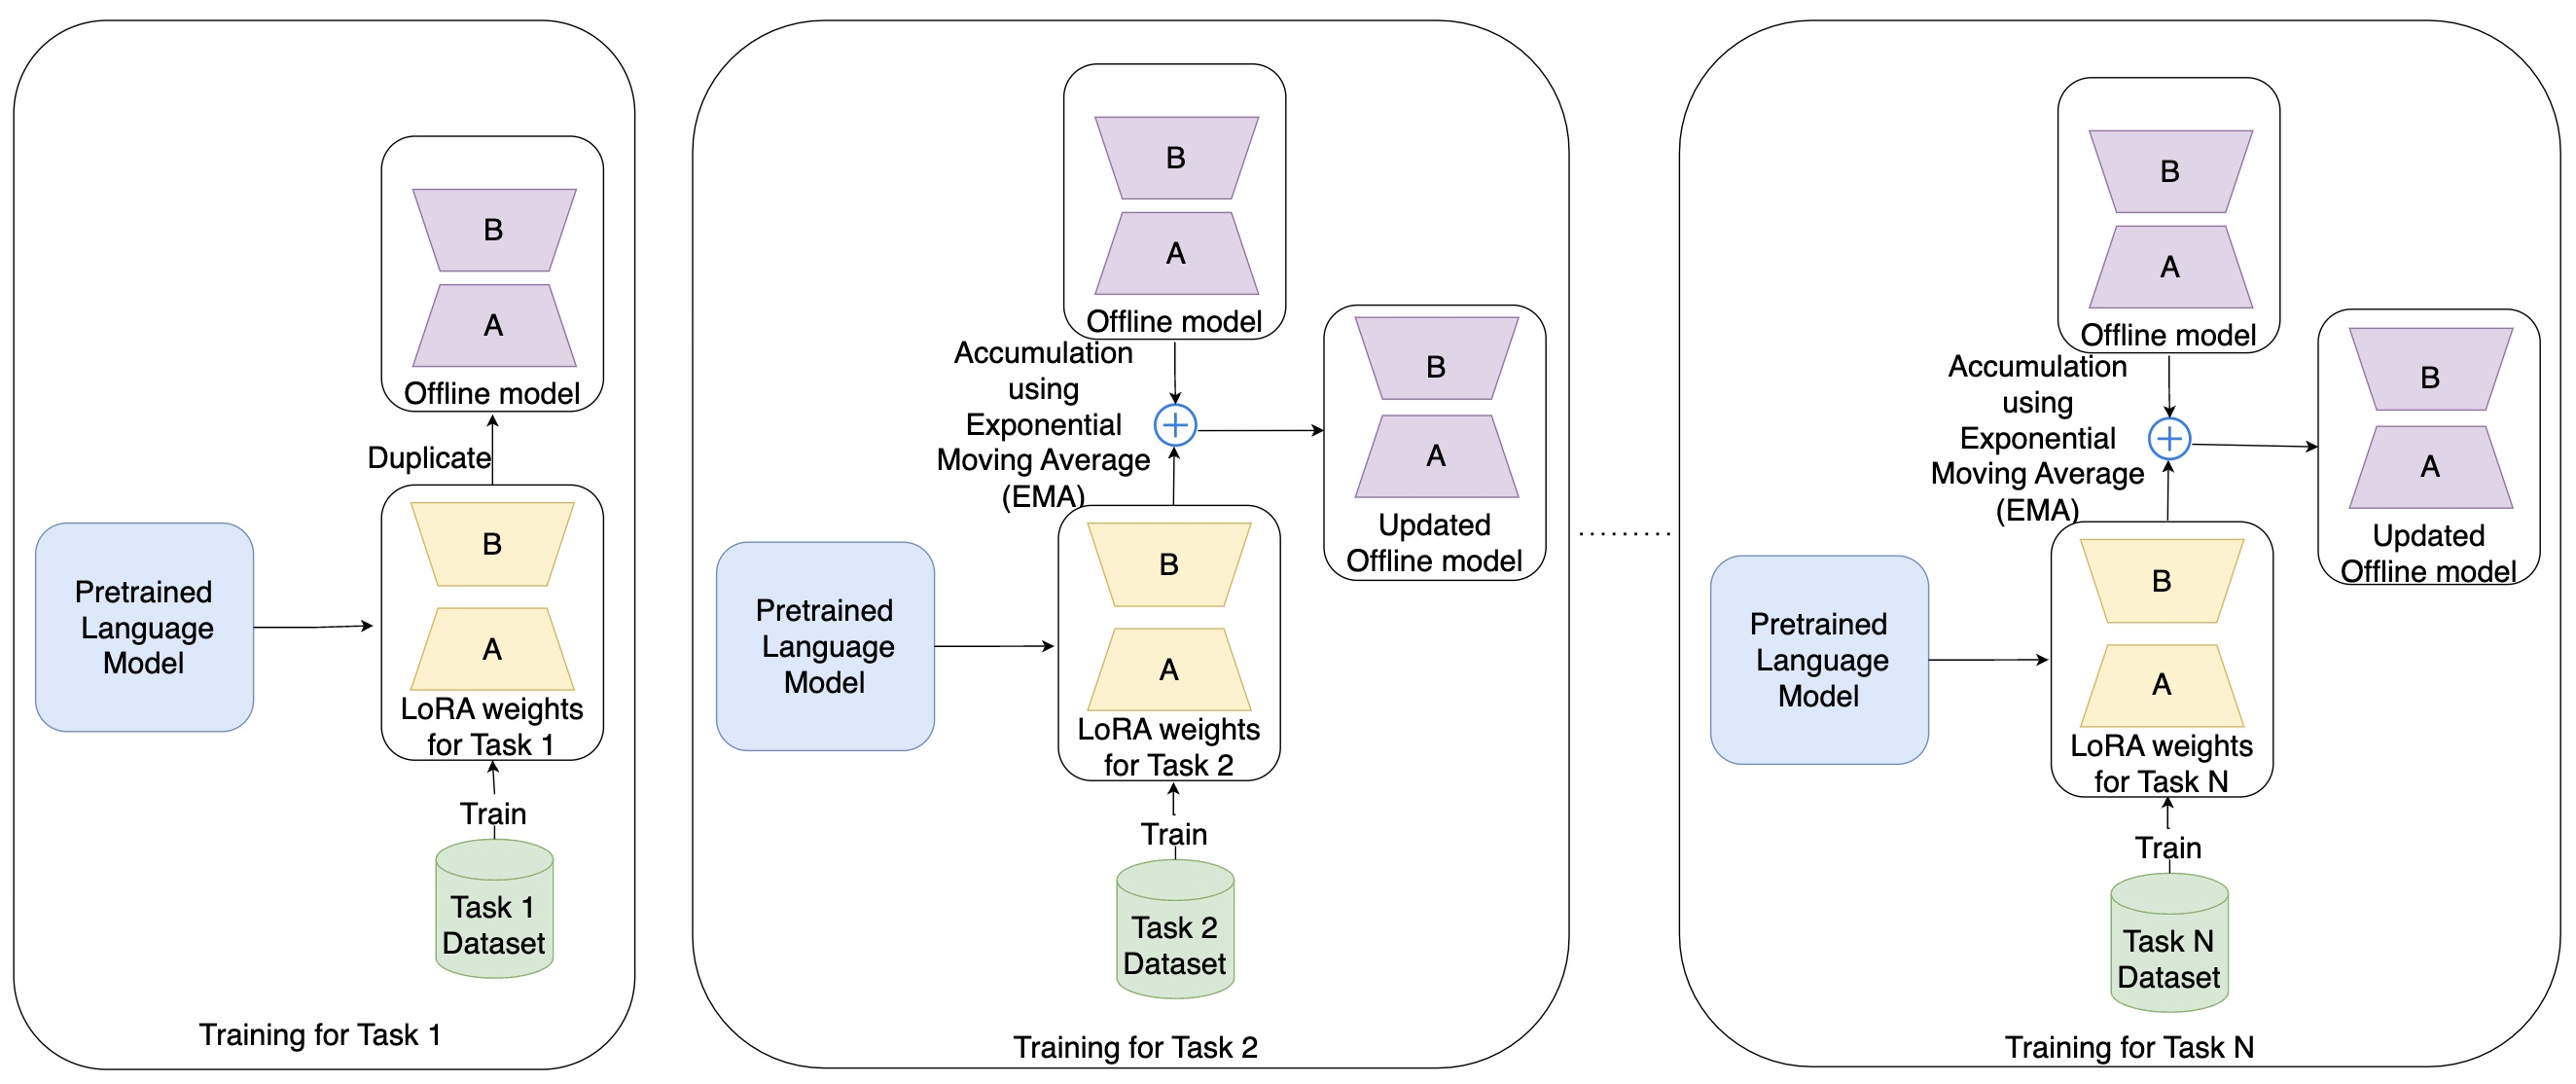
\includegraphics[width=1\textwidth]{Figures/literature_review/LAE.jpeg} 
    \caption{LAE Framework}
    \label{fig:LAE}
\end{figure}
\begin{enumerate}
\item Learning. Different PEFT modules have different adaptation speeds. Adapting a PEFT module to a task quickly can lead to overfitting and severe degradation of performance across tasks. Calibrating the PEFT modules to align their adaptation speeds for a new task by reducing the learning rate can help mitigate catastrophic forgetting.
\item Accumulation of multi-task knowledge. PEFT modules can be continuously trained to adapt to new tasks. However, this adaptation results in the forgetting of previously learned tasks. The LAE framework uses an additional offline expert to solve this issue. For a new task, a new online PEFT module is trained on the task. If it is the 1st task, the online module is duplicated to get the offline expert. Otherwise, the knowledge from the online module is accumulated in the offline expert using the accumulation function. 
\begin{equation}
\centering
\theta_{\text{peft}}^{\text{offline}} \leftarrow \alpha \cdot \theta_{\text{peft}}^{\text{offline}} + (1 - \alpha) \cdot \theta_{\text{peft}}^{\text{online}}
\end{equation}
where \(\alpha\) is a large weight decay.
\item Ensemble. The LAE framework uses an ensemble of the online PEFT module and the offline PEFT module to get the output.
\end{enumerate}
The LAE framework can be applied to any pre-trained model that is compatible with PEFT modules. 

\subsubsection{Inference Strategies to mitigate Catastrophic Forgetting}
There are some inference architectures that support learning incremental number of tasks while also mitigating catastrophic forgetting.

LoRAMoE \cite{dou2023loramoe} is a technique that uses LoRA adapters in a Mixture of Experts (MoE) architecture. MoE is an architecture which introduces multiple expert models. During supervised fine-tuning, the input data is routed to the most appropriate expert model based on the characteristics of the data using a routing function. This allows to adapt the processing to different data distributions. Increase in the amount of instruction data used for fine-tuning can continually change the model parameters, resulting in performance degradation and forgetting of the pre-trained knowledge. LoRAMoE addresses this by using multiple LoRA adapters as experts and a router to gate them in the feed forward neural network layer (FFN) of every transformer block. During the training process, the base model weights are frozen and only the LoRA adapters and the router are optimized. This ensures that only a small subset of parameters are updated for each task and limits interference with previously learned knowledge stored in other parameters. Thus, this helps prevent degradation of task-specific performance and forgetting of pre-trained knowledge. 
\begin{figure}[h]
    \centering
    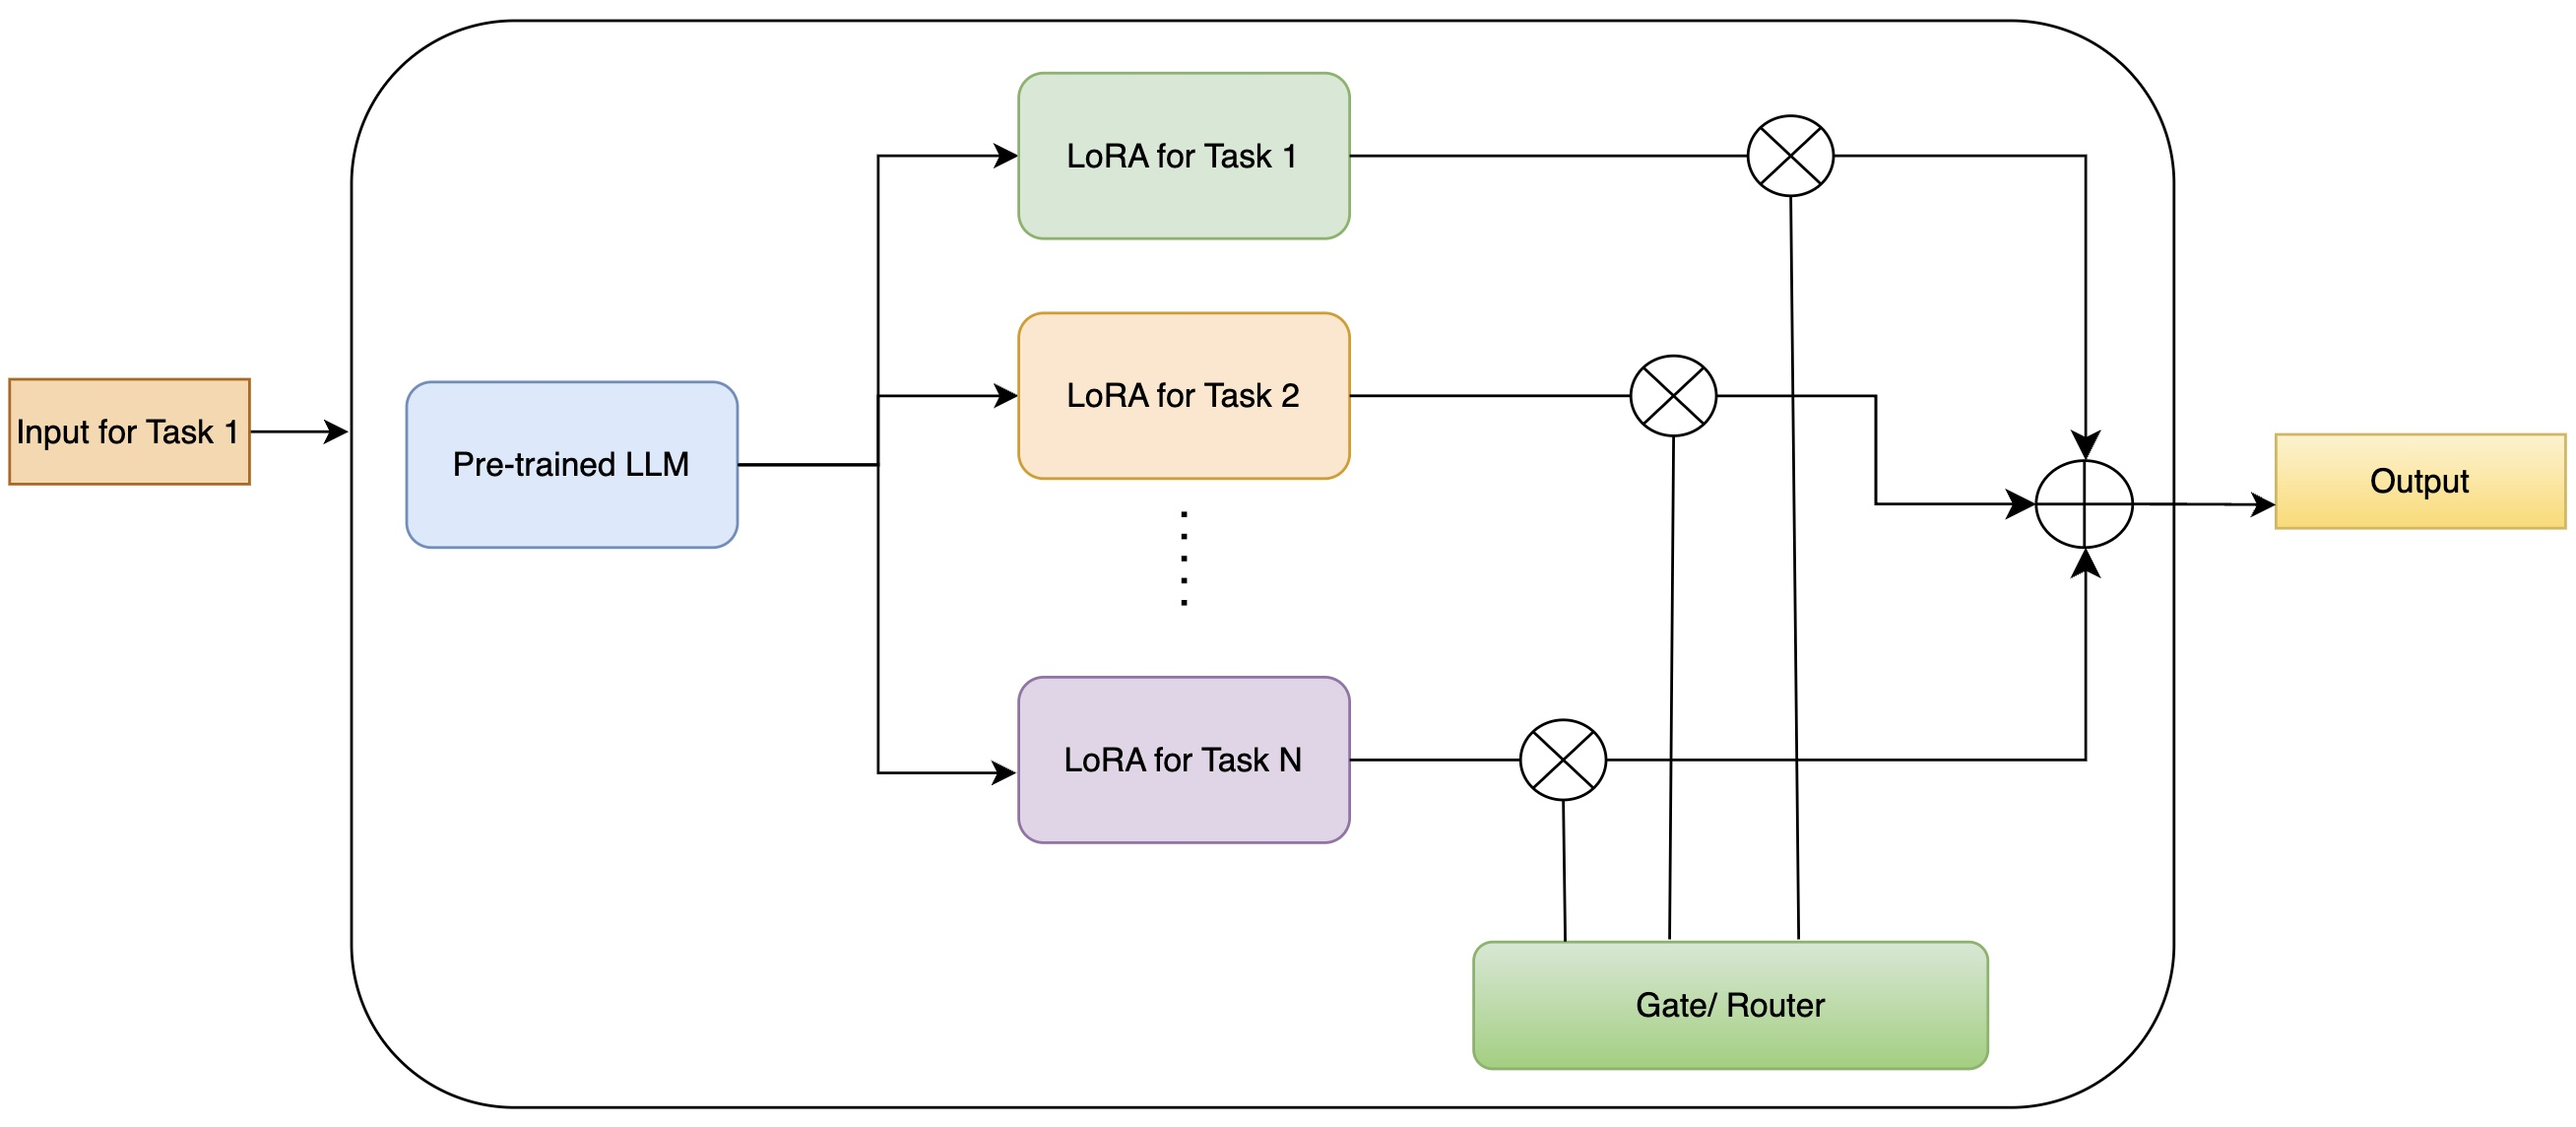
\includegraphics[width=1\textwidth]{Figures/literature_review/mixture_of_experts.jpeg} 
    \caption{Mixture of Experts with LoRA adapters}
    \label{fig:LoRAMoE}
\end{figure}

Scalable LoRA (S-LoRA) \cite{sheng2023s} is an approach developed for the scalable serving of many LoRA adapters. In this approach, all the LoRA adapters are stored in the main memory and unified paging is used to dynamically load the LoRA adapter to be used for the current task to the GPU memory. It uses batching for the computations of the base model and custom CUDA kernels for performing the low rank adaptation for the different LoRA adapters separately. This allows for efficient computation and parallelism of tasks. Using these features, it enables the scalable serving of many fine-tuned models trained on a variety of tasks.
\begin{figure}[h]
    \centering
    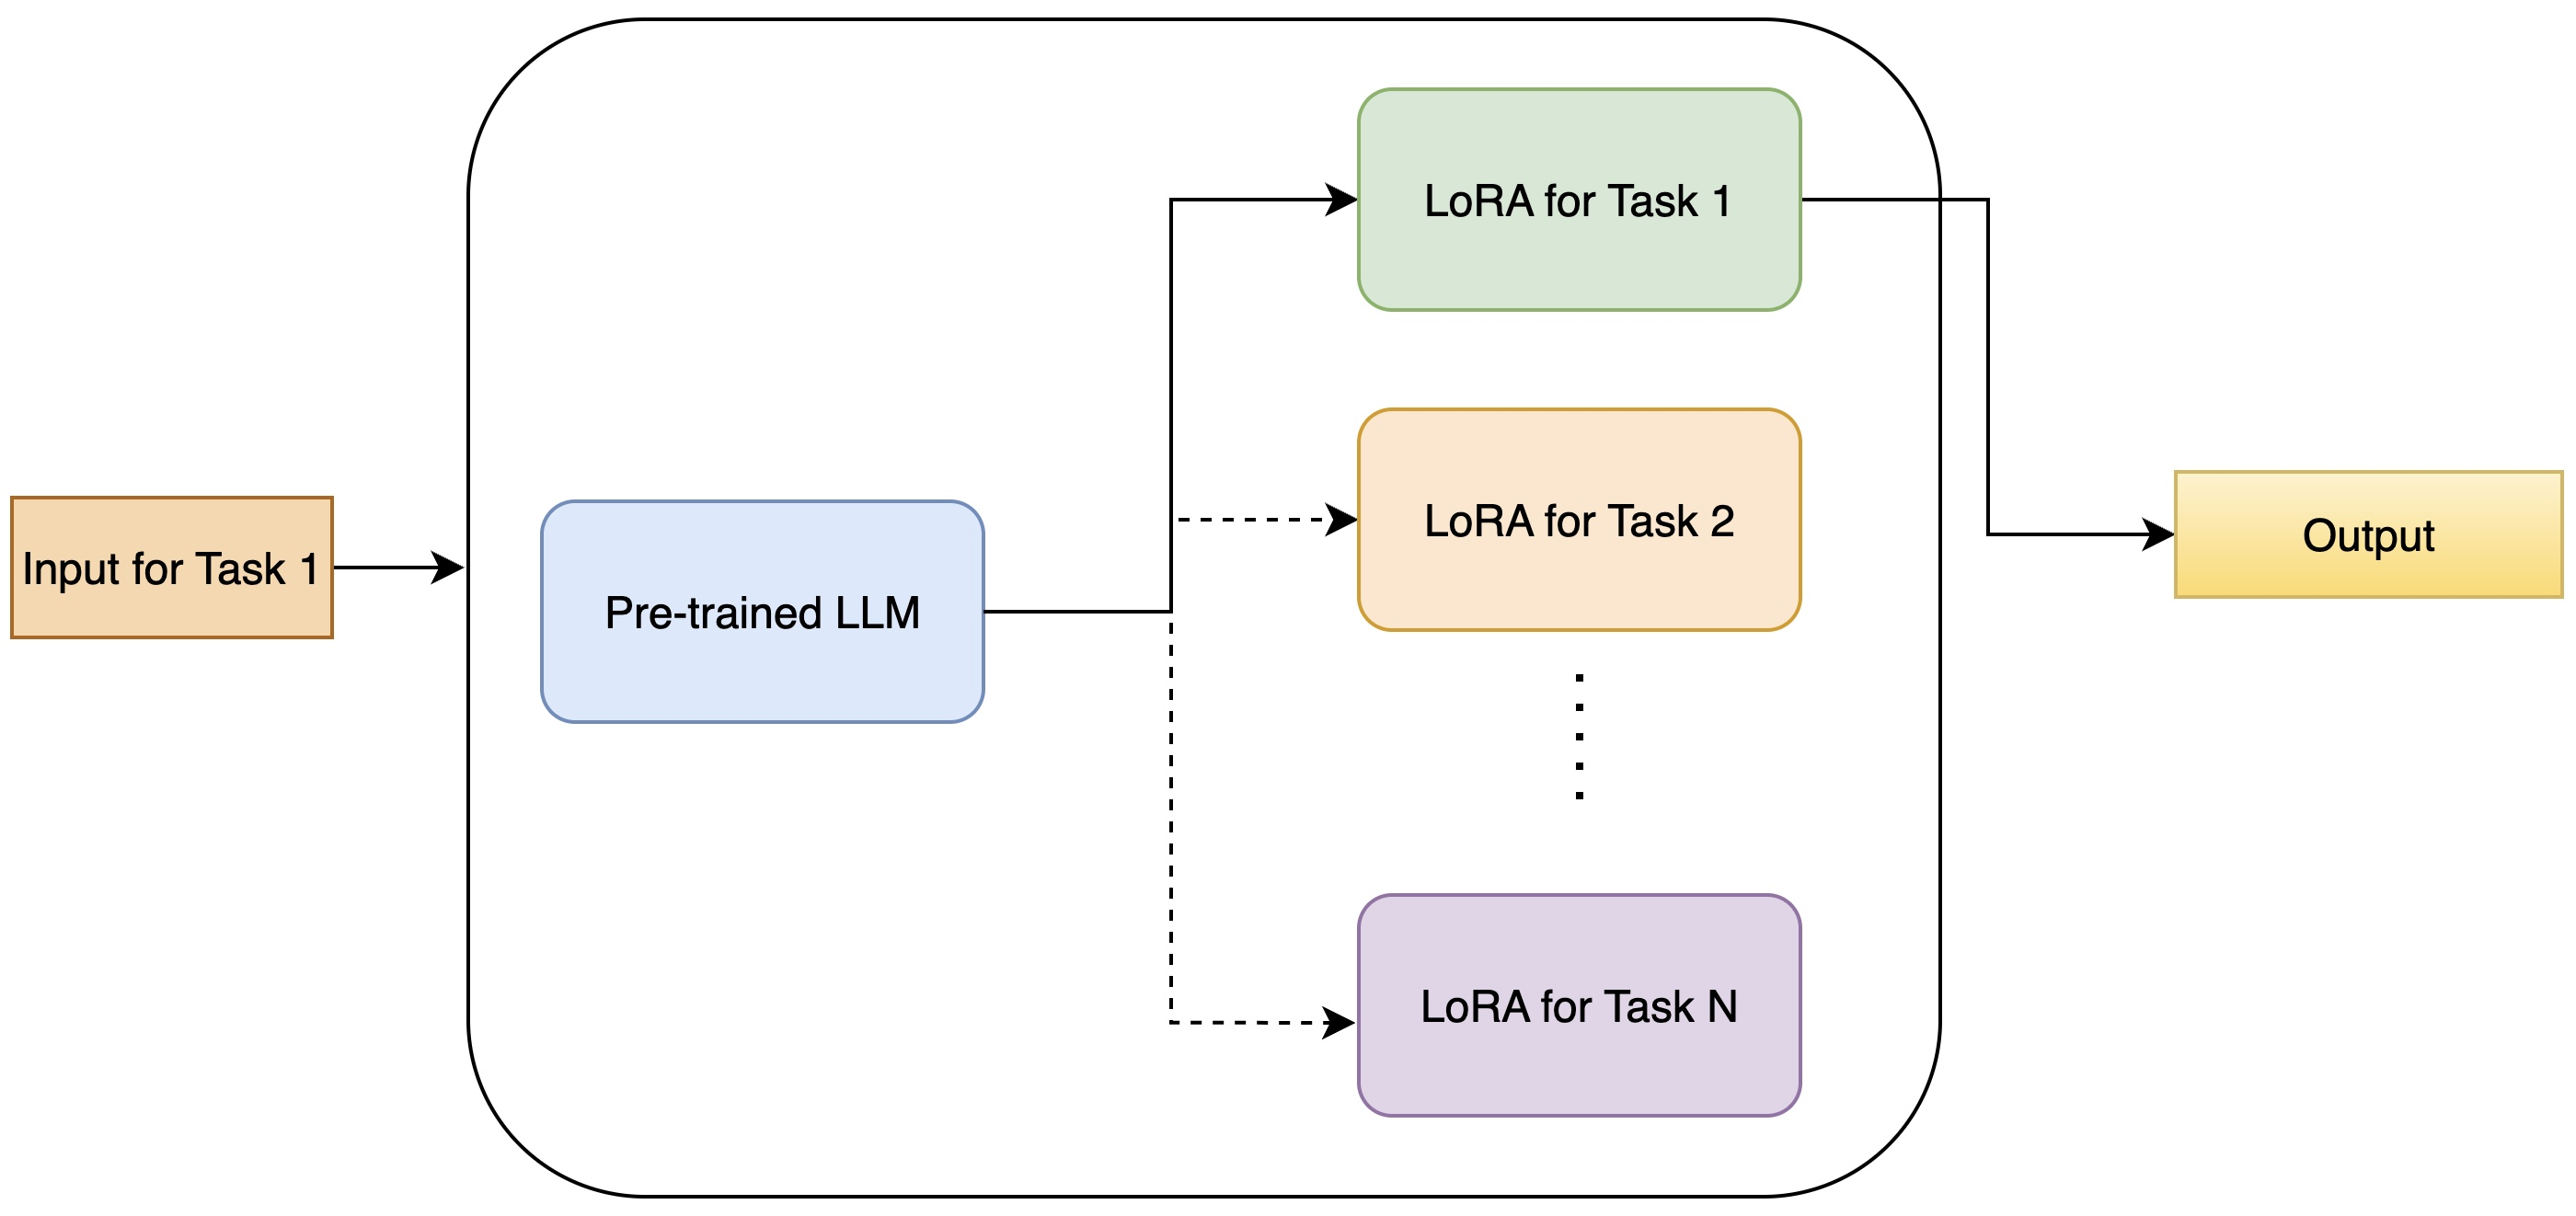
\includegraphics[width=1\textwidth]{Figures/literature_review/dynamic_loading.jpeg} 
    \caption{Dynamic Loading of LoRA adapters}
    \label{fig:SLoRA}
\end{figure}

Although these inference architectures have the potential to mitigate catastrophic forgetting by ensuring no interference between tasks, they bring the additional complexity of having to train a gating/ routing function for the dynamic selection of LoRA adapter for each input. Thus, our preference would be to have a single model with the capabilities to perform different tasks.

\subsection{Research gap and challenges}
Through this review of existing research and literature on continual learning, we identified several gaps in the existing body of knowledge. Many of the explored studies focused on preserving the model capabilities on previously learned tasks. Thus, there is a notable lack of emphasis on maintaining the pre-trained capabilities of the model in task-incremental learning. Furthermore, a lot of studies used classification tasks for their experiments. This does not adequately reflect the diverse nature of the tasks in real world applications. To address these limitations, this thesis work aims to bridge these gaps by:
\begin{enumerate}
    \item Investigating task-incremental learning and its impact on the pre-trained and task-specific capabilities of the model.
    \item Expanding the scope of the tasks used in the experiments, especially for code generation and natural language generation use cases.
    \item Using task-specific metrics and use case-specific benchmarks to accurately assess the impact of task-incremental learning on the model capabilities.
\end{enumerate}
Our approach seeks to provide a more comprehensive study that closely aligns with practical implementations, thereby enhancing the applicability of the findings.





%\section{Evaluation} 

\section{Metrics} \label{metrics}

Evaluation of LLMs is an important step in developing processes and building systems that use LLMs. Evaluation enables the identification of strengths and weaknesses of LLMs, thereby facilitating their further improvement and applications. Furthermore, the broad applicability of LLMs emphasizes the need for evaluation protocols to be put in place to ensure the safety and reliability of LLM-based systems \cite{chang2024survey}. The current LLMs are versatile and are capable of performing various tasks. Thus, LLMs need to be evaluated using a multifaceted approach on language understanding, generation, reasoning, and task-specific performance. Most LLMs report evaluation results on standard benchmarks such as ARC \cite{clark2018think}, GSM8K \cite{zhang2024careful}, GLUE (General Language Understanding Evaluation) \cite{wang2018glue}, and HellaSwag \cite{zellers2019hellaswag}. 


%\subsection{Metrics} \label{metrics}

These evaluations use different metrics to measure performance across different dimensions and task capabilities. 


\subsection{pass@k} \label{pass@k}
The pass@k metric is defined as the probability that at least one of the top k-generated samples for a problem is correct \cite{chen2021evaluating}. It is used to check the functional correctness of code samples. The following steps are followed to compute pass@k:
\begin{enumerate}
\item Generate n>=k responses for each code problem.
\item Count the number of correct responses (c) which pass the unit tests prepared for that code problem.
\item Compute pass@k using the formula:
\end{enumerate}
\begin{equation}
\text{pass@k} = E_{\text{problems}} \left[ \frac{1 - C(n-c,k)}{C(n,k)} \right]
\end{equation}

where
\begin{align*}
n &\text{ is the total number of samples} \\
C &\text{ = Combination} \\
c &\text{ is the number of correct samples} \\
k &\text{ is the number of top samples considered} \\
E &\text{ denotes the expected value over the problems}
\end{align*}




\subsection{BLEU} \label{bleu}
The Bilingual Evaluation Understudy (BLEU) score is a metric for evaluating a generated sentence to a reference sentence \cite{papineni2002bleu}. It is an evaluation metric created for Machine Translation tasks. It is computed by comparing the n-grams of the translated (candidate) sentence to the n-grams of the reference human-translated sentence. It is a precision-based measure. The score ranges from 0 to 1. The higher the score, the better the quality of the generated response.
\begin{equation}
\text{BLEU score} = BP \cdot \exp\left( \sum_{i=1}^{N} (w_i \cdot \ln(p_i)) \right)
\end{equation}

where
\begin{align*}
BP &\text{ is Brevity Penalty} \\
w_i &\text{ is the weight for n-gram precision of order } i. \\
p_i &\text{ is the n-gram modified precision score of order } i. \\
N &\text{ is the maximum n-gram order to consider.}
\end{align*}

Brevity Penalty penalizes the predictions that are too short compared to the reference sentences. It is computed using:
\begin{equation}
BP = 
\begin{cases}
1, & \text{if } c > r \\
e^{(1 - r/c)}, & \text{if } c \leq r
\end{cases}
\end{equation}

where
\begin{align*}
c &\text{ is the length of the candidate code.} \\
r &\text{ is the effective reference corpus length.}
\end{align*}
For computing the modified precision score p\_i, we count the number of n-grams matched with the references for all the candidate responses in the dataset. We divide this count by the sum of the count of all n-grams in the references to get the score. It is computed using the formula:
\begin{equation}
p_n = \frac{\sum_{C \in \text{Candidates}} \sum_{i=1}^{l} \mu_n^i \cdot \text{Count}_{\text{clip}} (C(i,i+n))}{\sum_{C' \in \text{Candidates}} \sum_{i=1}^{l} \mu_n^i \cdot \text{Count}_{\text{clip}} (C'(i,i+n))}
\end{equation}

where:
\begin{align*}
n &\text{ is the length of the n-gram.} \\
C(i, i+n) &\text{ is the n-gram from position } i \text{ to position } i+n. \\
\text{Count}_{\text{clip}}(C(i, i+n)) &\text{ is the maximum number of n-grams occurring in a } \\
&\text{ candidate code and a set of reference codes.} \\
\mu_n^i &\text{ is the weights of different keywords or n-grams.}
\end{align*}



\subsection{CodeBLEU} \label{codebleu}
The BLEU metric evaluates Machine Translation tasks well. However, it does not work well for code synthesis tasks. The CodeBLEU metric extends the BLEU metric for code generation by including syntactic and semantic characteristics. The CodeBLEU score is a weighted combination of n-gram match (BLEU), weighted n-gram match (BLEU-weighted), AST match and Data flow match scores \cite{ren2020codebleu}.
\begin{equation}
\text{CodeBLEU score} = \alpha \cdot \text{BLEU} + \beta \cdot \text{BLEU}_{\text{weight}} + \gamma \cdot \text{Match}_{\text{ast}} + \delta \cdot \text{Match}_{\text{df}}
\end{equation}

The components in the formula are described as follows:
\begin{enumerate}
\item BLEU is the BLEU metric score.
\item $BLEU_{weight}$ is the weighted n-gram match score. It is a weighted version of the BLEU score, where keywords have higher weights than other words. The weighted n-gram match score is computed using the formula:
\begin{equation}
\text{BLEU}_{\text{weight}} = BP \cdot \exp\left( \sum_{n=1}^{N} w_n \log p_n \right)
\end{equation}
\item $Match_{ast}$ is the Syntactic Abstract Syntax Tree (AST) match. It is an accuracy measure calculated by comparing the reference and candidate syntax sub-trees while ignoring the leaves since they represent variable or function names. It is computed using:
\begin{equation}
\text{Match}_{\text{ast}} = \frac{\text{Count}_{\text{clip}}(T_{\text{cand}})}{\text{Count}(T_{\text{ref}})}
\end{equation}
where
\begin{align*}
\text{Count}(T_{\text{ref}}) &\text{ is the total number of the reference subtrees} \\
\text{Count}_{\text{clip}}(T_{\text{cand}}) &\text{ is the number of the candidate subtrees that are matched with} \\
&\text{the reference.}
\end{align*}

\item $Match_{df}$ is Semantic Data Flow Match. It is a metric that evaluates the semantic differences between the reference and a candidate using the data flow. The data flow is a graph where variables represent nodes, and their source represents the edges. It is computed using the formula:
\begin{equation}
\text{Match}_{\text{df}} = \frac{\text{Count}_{\text{clip}}(\text{DF}_{\text{cand}})}{\text{Count}(\text{DF}_{\text{ref}})}
\end{equation}
where
\begin{align*}
\text{Count}(\text{DF}_{\text{ref}}) &\text{ is the total number of the reference data-flows,} \\
\text{Count}_{\text{clip}}(\text{DF}_{\text{cand}}) &\text{ is the number of matched candidate data-flows.}
\end{align*}

\item \[
\alpha, \beta, \gamma, \text{ and } \delta \text{ are the weights for each term in the formula.}
\]
\end{enumerate}


\subsection{Accuracy/ Exact Match} \label{accuracy}
Exact Match is a simple metric to check if the model’s generated answer exactly matches the true answer \cite{wu2023online}. The exact match score is 1 if the generated response completely matches the reference answer, and 0 if not. The final Exact Match score is computed using the formula:
\begin{equation}
\text{Exact Match} = \frac{\text{Number of exact matches}}{\text{Total number of samples}}
\end{equation}

\subsection{ROUGE-L} \label{rougel}
ROUGE (Recall-Oriented Understudy for Gisting Evaluation) is a set of metrics used for evaluating summarization and machine translation tasks \cite{lin2004rouge}. ROUGE-L is a variant of ROUGE, which measures the longest common subsequence (LCS) between the model generation and the reference text. It computes precision, recall and F1-score based on the length of the longest common subsequence. The LCS can be computed on either on a sentence-level or a summary-level.
Given the model generated answer and reference answer for a question, ROUGE-L is computed as follows:
\begin{enumerate}
\item Tokenize the answers to get generated tokens and reference tokens.
\item Get the length of the longest common subsequence (lcs\_length) between the two.
\item Use the formulas:
\begin{align*}
\text{Precision} &= \frac{\text{lcs\_length}}{\text{length of generated\_tokens}} \\
\text{Recall} &= \frac{\text{lcs\_length}}{\text{length of ground\_truth\_tokens}} \\
\text{F1score} &= \frac{2 \times \text{Precision} \times \text{Recall}}{\text{Precision} + \text{Recall}}
\end{align*}
\end{enumerate}

\subsection{Measuring forgetting across tasks}
Task-incremental continual learning involves measuring performance across a sequence of tasks. In our investigation of the effects of task-incremental learning on model capabilities, it is important to measure catastrophic forgetting and the impact of task-specific fine-tuning on overall model performance. In continual learning, evaluation requires assessing the performance of the fine-tuned model on new tasks as well the retention of previously learned tasks. The following metrics can be employed for performance evaluation.

\subsubsection{Backward Transfer (BWT)} \label{bwt}
Backward Transfer measures the performance degradation on prior tasks after a model has been trained on new tasks \cite{wu2023online}. It provides a measure of the model’s retention ability.
\begin{equation}
\text{BWT}_T = \frac{1}{T-1} \sum_{i=1}^{T-1} \left( a_{T,i} - a_{i,i} \right)
\end{equation}

where:
\begin{itemize}
\item \( T \) is the task count,
\item \( a_{T,i} \) is the performance of the model on the test set of task \( t_i \) after training on the task \( t_T \),
\item \( a_{i,i} \) is the performance of the model on the test set of task \( t_i \) after training on the task \( t_i \).
\end{itemize}


\subsubsection{Forward Transfer (FWT)} \label{fwt}
Forward Transfer measures the positive impact on the performance of new tasks when a model has completed training on preceding tasks \cite{wu2023online}.
\begin{equation}
\text{FWT}_T = \frac{1}{T-1} \sum_{i=2}^{T} a_{i-1,i}
\end{equation}

where \( a_{i-1,i} \) is the score of the model on the test set of task \( t_{i-1} \) after training on task \( t_i \).



\section{Benchmarks} \label{benchmarks}
Benchmarks are standardized frameworks for conducting a comprehensive evaluation of an LLM's performance. Benchmarks provide quantitative measures that highlight the strengths of an LLM and its areas for improvement. A thorough LLM evaluation requires using several benchmarks to assess its overall performance. When the intended application is known, it is important to select task-specific benchmarks that align well with the targeted task to measure its capabilities on that task. The following are different benchmarks that have been widely adopted for the evaluation of code generation and natural language generation tasks.

\subsection{HumanEval} \label{humaneval}
The \href{https://huggingface.co/datasets/openai/openai_humaneval}{HumanEval benchmark} \cite{chen2021evaluating} is a dataset designed to evaluate the code generation capabilities of LLMs. It is composed of 164 hand-written problems written in Python with each sample including a function and several unit tests for that function. It is used to measure the functional correctness of the code generated by the LLMs by checking if the generated code passes the unit tests. The pass@k metric is used for the performance evaluation of this benchmark.

\subsection{MultiPL-E} \label{multiple}
\href{https://huggingface.co/datasets/nuprl/MultiPL-E}{MultiPL-E} is a dataset for evaluating the code generation capabilities of LLMs on 18 different programming languages. It takes the problems from HumanEval and MBPP Python benchmark and uses compilers to translate them to other languages. DeepSeek-Coder uses this dataset for its code generation evaluation on C++, Java, PHP, TypeScript, C\#, Bash, and JavaScript. The pass@k metric is used for the performance evaluation for this benchmark.

\subsection{HumanEval-X} 
\href{https://huggingface.co/datasets/THUDM/humaneval-x}{HumanEval-X} is a benchmark for evaluating the code generation capabilities of LLMs on multiple programming languages. It consists of 820 hand-written problems written in Python, Java, C++, Go and JavaScript. Like HumanEval, each sample contains a function and several unit tests for that function. The pass@k metric is used for the performance evaluation for this benchmark.

\subsection{CoNaLa} \label{conala}
The \href{https://huggingface.co/datasets/neulab/conala}{Code/ Natural Language Challenge (CoNaLa)} is a dataset designed to test systems for generating code from natural language. It is a benchmark for code and natural language pairs. The dataset was prepared by crawling code samples from Stack Overflow and then curated by annotators to get 2379 training and 500 test samples in Python. This dataset is used to evaluate code generation capabilities of LLMs.

\subsection{ARC} \label{arc}
The \href{https://allenai.org/data/arc}{AI2 Reasoning Challenge (ARC)} \cite{clark2018think} is a benchmark dataset containing 7787 grade-school level multiple-choice science questions. The dataset was prepared for advancing question-answering systems. The dataset is partitioned into a Challenge set and an Easy set. The datasets are further split into train, test, and development sets, as shown in table \ref{tab:arc}. This benchmark is designed to evaluate the reasoning capabilities of LLMs.

\begin{table}
\centering
\caption{Data splits for ARC benchmark dataset}
\label{tab:arc}
\begin{tabular}{|c|c|c|} \hline
 & Challenge Set & Easy Set \\ \hline
Train & 1,119 & 2,251 \\ \hline
Test & 1,172 & 2,376 \\ \hline
Development & 299 & 570 \\ \hline
\end{tabular}
\end{table}

\subsection{GSM8K} \label{gsm8k}
\href{https://huggingface.co/datasets/openai/gsm8k}{Grade School Math 8K (GSM8K)} \cite{zhang2024careful} is a benchmark dataset containing 8.5K grade school math word problems. This dataset was prepared to support the task of basic mathematical problems that need multi-step reasoning. This dataset is used to
evaluate the math and logic capabilities of LLMs.

\subsection{BoolQ} \label{boolq}
\href{https://huggingface.co/datasets/google/boolq}{BoolQ} \cite{clark2019boolq} is a question-answering benchmark dataset for yes/ no questions. It contains 15942 samples with each sample containing question, passage, and answer. The BoolQ dataset is used to evaluate the reading comprehension capabilities of LLMs.





